
Comme définit dans le chapitre précédent, ce problème concerne deux problèmes dépendants : attribuer les missions aux chariots cavaliers et calculer les dates d'exécution de ces missions de façon à minimiser une fonction de coût. 
Nous détaillerons dans ce chapitre les caractéristiques du problème et nottament l'impact de la dynamique et de l'incertitude vis-à-vis de la résolution, puis nous proposerons deux modélisations possibles faisant le lien avec le contexte théorique détaillé dans le premier chapitre. Enfin nous décrirons les méthodes de résolution élaborées durant cette thèse et permettant de proposer des solutions de façon dynamique. Il sera question d'une méthode de résolution exacte d'une part, puis de plusieurs méthode de résolution approchée d'autre part. Plusieurs heuristiques seront ainsi présentées et deux méthodes utilisant la métaheuristique fourmi seront décrites.

\section{Dynamique et incertitude}

\subsection{Gestion du temps}

Pour plus de simplicité nous choisissons de considérer le problème sur une période de temps fixée que nous appellerons journée. Il est à noter que dans la plupart des terminaux, l'exploitation ne s'arrête jamais. Cette utilisation continue est la raison pour laquelle une modélisation statique du problème est totalement inapplicable.

Néanmoins, une partie des missions à réaliser sont connues bien à l'avance et peuvent être ainsi plus facilement allouées aux chariots cavaliers. Au contraire d'autres missions ne sont connues qu'une fois la journée d'exploitation débutée et doivent être ordonnancées en tenant compte des calculs précédents.

Dans le cadre du problème d'affectation des missions aux chariots cavaliers, la notion de degré effectif de dynamicité de Larsen (voir \ref{subsec:dynamique}) permettant de définir la difficulté induite par la dynamique d'un jeu de données devra être adaptée. En effet, la difficulté à ordonnancer une mission est associée à l'écart de temps entre la date de l'arrivée de la mission dans le système de planification et la date de début au plus tard de la mission, c'est-à-dire la date au delà de laquelle la fenêtre de temps ne pourra plus être respectée. Ainsi, plus une mission est connue en avance, plus elle est facile à ordonnancer. En revanche une mission qui est connue au dernier moment doit être immédiatement insérée dans le plan de charge d'un véhicule afin de pouvoir être accomplie dans les temps. Définissons ainsi $\eta$ le nombre de missions à réaliser, $t_i$ ($1 \leq i \leq \eta$) la date d'arrivée de la $i^{\text{ème}}$ mission dans le système et $T_i$ sa date de début au plus tard. Le degré effectif 
de dynamicité peut donc être définit selon la formule suivante : 

\begin{equation}
 edod = \frac{\sum \limits_{i=1}^{\eta}\left( \frac{t_i}{T_i} \right)}{\eta}
\end{equation}

Selon cette formule, le degré effectif de dynamicité peut être supérieur à 1 si une ou plusieurs mission sont connues après leur date de début au plus tard. Dans ce cas, les contraintes de temps ne pourrons pas être respectées mais la mission devra quand même être planifiée en cherchant à minimiser le retard.


\subsection{Incertitude}
En plus de la notion de dynamicité, il existe de l'incertitude sur les données des missions. L'incertitude peut se situer à différents niveaux.

\subsubsection{Incertitude liée aux clients du terminal}

Le bassin du Terminal de Normandie est un bassin à marée, c'est-à-dire que la hauteur de l'eau dépend de la marée et donc que les fenêtres de temps d'arrivée et de départ des portes-conteneurs suivent un rythme d'un peu plus de 12 heures.
Si un porte-conteneurs manque la marée, ne serait-ce que d'une heure, il devra attendre la marée suivante au large face à l'entrée du port. Dans ce cas, les missions de déchargement/chargement du navire prévues à l'avance seront annulées et devrons être planifiées à nouveau afin de prendre en compte les nouveaux horaires de présence du porte-conteneurs à quai. Ce décalage des missions aura des conséquences sur les autres missions du terminal et une planification globale devra être calculée.
D'autre part, si le chargement du navire est retardé dans le terminal, son départ peut être décalé à la marée suivante. Dans ce cas le terminal devra verser des pénalités à l'armateur du navire.

Concernant les camions, les heures d'arrivées sont souvent connues à l'avance mais sont sujettes aux variations du trafic. Ainsi, au Havre les voies d'accès au port empruntent différents ponts-levant. Si les ponts sont abaissés, les camions seront à l'heure. En revanche un pont levé peut retarder les camions de plusieurs dizaines de minutes. D'autres camions ne sont parfois pas prévus dans le registre du terminal et doivent être tout de même servis. Le système d'affectation des missions doit être suffisamment flexible afin de permettre d'intégrer ces missions dans les plans de charge des chariots cavaliers pour répondre aux demandes dynamiques.
Si un camion, présent à l'heure sur le terminal n'est pas servi dans les temps par un chariot cavalier, le terminal devra payer des frais de pénalité au transporteur.

Grâce à un réseau ferré développé et à un trafic maîtrisé, les trains sont moins sujets aux retards, ou du moins, ceux-ci sont annoncé à l'avance. En revanche, si les wagons ne sont pas chargés/déchargés à temps, le terminal devra également payer des pénalités.

\subsubsection{Incertitude liée aux chariots cavaliers}

La seconde source d'incertitude est liée aux chariots cavaliers à travers leurs pannes et leurs conducteurs.

\paragraph{Panne des chariots cavaliers}
%Panne
Comme détaillé dans le chapitre précédent, un chariot cavalier est un engin mécanique soumis à d'énorme contraintes physiques. 
Afin d'éviter des pannes, une maintenance régulière et approfondie est effectuée. Ainsi, la totalité de la flotte n'est que rarement disponible pour l'exploitation. Néanmoins, il arrive qu'un chariot cavalier tombe en panne et doive être réparé.

Une panne peut concerner soit la partie fille du chariot, c'est-à-dire le système de levage (\textit{spreader}), soit la partie mère c'est-à-dire le chariot en lui-même (partie moteur, train roulant, système électrique, etc), soit les deux à la fois. 
En fonction du type de panne la réparation peut être réalisée sur place ou nécessitera un passage par le dépôt. 
Dans le cas d'une panne empêchant le déplacement autonome du chariot, un remorquage sera nécessaire. Toutes ces opérations de retour au dépôt, réparation, retour sur zone d'exploitation, provoquent un retard à la fois lié à l'indisponibilité du véhicule et à l'inaccessibilité de la travée sur laquelle le véhicule est tombé en panne.

Si la panne concerne le système de levage, il existe deux cas de figure. D'une part, le conteneur à déplacer n'a pas pu être chargé sur le chariot cavalier et dans ce cas le chariot sera réparé et pendant ce temps la mission sera réaffectée à un autre véhicule. D'autre part, le conteneur a déjà été soulevé par le chariot cavalier et dans ce cas il faudra attendre la réparation du véhicule avant de pouvoir décharger le conteneur à nouveau.

\paragraph{Facteur humain}
%Non respect de la mission affectée + Perte de conteneurs
Les chariots cavaliers sont pilotés par des opérateurs qui agissent selon leurs propres décisions. 
Lorsqu'un conducteur est disponible il demande au système de planification une liste de missions à effectuer. 
Le système lui fourni ainsi un plan de charge à respecter. 
Néanmoins, le conducteur peut décider de respecter ce plan ou non. 
Il indique au système chaque nouvelle mission débutée afin de mettre à jour la base de données et d'avertir les autres conducteurs de chariots cavaliers de son intention (ceci évite de mobiliser deux véhicules pour une même mission). 
Cependant, il arrive que le conducteur indique réaliser une mission alors qu'il en effectue une autre. 
De même, il peut oublier d'indiquer la réalisation d'une mission lorsque celle-ci est terminée. 
Le système considère alors dans le premier cas que le conteneur de la mission a été déplacé, et dans le second cas que le conteneur est toujours au même endroit. 
Tous ces comportements provoquent des incohérences dans le système qui conduisent bien souvent à des pertes de conteneurs. 
Des agents sont donc chargés de se déplacer à pieds dans les gigantesques travées du terminal afin de rechercher les conteneurs perdus.

%Non respect d'itinéraire
D'autre part, lorsqu'un conducteur valide son intention de réaliser une mission, le système lui propose un itinéraire à suivre afin d'atteindre le point de collecte, puis le point de livraison du conteneur. 
Dans le cadre de la gestion du trafic sur le terminal, le système de routage peut tenir compte de la présence d'autres véhicules afin de minimiser les temps d'attente en entrée de travée. 
Lorsque le conducteur débute sa mission, les travées qu'il va emprunter sont ainsi réservées afin d'empêcher un autre chariot de les emprunter au même moment. 
De même, l'itinéraire est calculé afin de permettre au véhicule d'éviter les zones congestionnées et donc d'arriver à l'heure prévue par le système. 
Si le conducteur ne respecte pas cet itinéraire, il peut arriver en retard (ou parfois en avance) à l'entrée de la travée ce qui peut provoquer un engorgement du fait du non respect de la période de réservation de cette travée.\\

En plus de la complexité naturelle du problème, la dynamique et l'incertitude viennent troubler les solutions calculées. Il est ainsi difficile d'envisager de le résoudre de façon exacte. La durée de validité de la solution ainsi calculée pourrait être inférieure à son temps de calcul. Une solution approchée, suffisamment performante, devra être calculée tout en tenant compte de la dynamique et de la méconnaissance de certaines parties du problème.


\section{Modélisations du problème}

Le problème peut-être abordé sous plusieurs formes. La première consiste à le modéliser sous forme d'un problème de tournées de véhicules. C'est la représentation la plus naturelle d'un problème utilisant des véhicules. La seconde modélisation est de considérer un problème d'atelier.

\subsection{Problème de tournées de véhicules}\label{chapitre:ordo:sec:modelisation:subsec:vrp}

Comme décrit précédemment, le problème de tournées de véhicules est une spécialisation du problème du voyageur de commerce où une série de lieux doivent être visités par des véhicules de la flotte. Dans ce problème, deux véhicules différents ne peuvent pas visiter une même ville et une ville ne peut-être visitée qu'une seule fois. L'objectif est de minimiser la distance totale parcourue tout en respectant les contraintes de capacité de chaque véhicule.


%Voyageurs
Concernant l'application aux chariots cavaliers et aux terminaux à conteneurs, le problème se caractérise dans le cas général par des véhicules à capacité unitaire. La non possibilité de transporter plusieurs conteneurs simplifie le problème qui se révèle appartenir au problème des multiples voyageurs de commerce à $m$ voyageurs (où $m$ est égal au nombre de véhicules). 


La flotte de véhicules peut-être homogène ou hétérogène. Nous considérerons le cas le plus général, c'est-à-dire en conservant la possibilité de rencontrer des véhicules de différents types. Dans ce cas, il est indispensable de distinguer les véhicules les uns des autres. Définissons ainsi $M$ l'ensemble des voyageurs de commerce (et donc par extension l'ensemble des véhicules) et le $k^{\text{ème}}$ voyageur $m_k$ ($\forall$ $k$ $\in$ $[1;m]$).

Dans le problème théorique les véhicules (ou les voyageurs de commerce) débutent tous leur tournée du dépôt et y retournent à la fin de leur tournée. Dans notre problème, les tournées peuvent être calculées en plein milieu d'une journée d'exploitation du terminal. Ainsi, les véhicules débutent leur tournée depuis l'emplacement où ils se trouvent s'ils sont inactifs, ou depuis l'emplacement où ils se trouveront à la fin de leur activité courante dans le cas contraire.

%Villes
D'autre part, une mission correspond à une ville à visiter par l'un des voyageurs de commerce. Soit $N$ l'ensemble des villes à visiter et $n_i$ la ville de la $i^{\text{ème}}$ mission à effectuer ($\forall$ $i$ $\in$ $[1;n]$) plus $n_0$ le dépôt. Chaque ville $i$ doit être visitée en respectant deux fenêtres de temps (\textit{Time Windows}) $TW_{i,1}$ et $TW_{i,2}$ respectivement de collecte et de livraison. $TW_{i,1}^{\min}$ et $TW_{i,1}^{\max}$ correspondent au minimum et au maximum de la fenêtre de temps $TW_{i,1}$.

\subsubsection{Structure du graphe}
%Graphe
Ce problème est ainsi modélisé par un graphe complet où les n\oe{}uds sont les missions (villes) et où les arcs correspondent à l'enchaînement de deux missions. 
Définissons ainsi $G^{(t)}=(V,A)$ le graphe complet où $V$ est l'ensemble des villes (plus le dépôt des véhicules) et $A$ est l'ensemble des arcs.

\begin{figure}[h]
\begin{center}
 \begin{tikzpicture}[xscale=5,yscale=5,->,shorten >=2pt,shorten <=2pt, auto,inner sep=2pt,semithick,bend angle=10]
    \tikzstyle{every state}=[circle,draw,fill=white,line width=0.5pt,minimum size=22pt,inner sep=0pt,font=\tiny]
    \node[state] (depot) at (1,1) {$depot$};
    \node[state] (v_3) at (0,1)      {$v_3$};
    \node[state] (v_2) at (0,0)      {$v_2$};
    \node[state] (v_1) at (1,0)      {$v_1$};
    \path (depot) edge [bend right,looseness=0.9] node[font=\tiny, black,sloped,above] {$c^k_{(\text{depot},v_1)}$}            (v_1)
		  edge [bend right,looseness=0.9] node[font=\tiny, black,sloped,above,near start] {$c^k_{(\text{depot},v_2)}$}            (v_2)
		  edge [bend right,looseness=0.9] node[font=\tiny, black,sloped,above] {$c^k_{(\text{depot},v_3)}$}            (v_3)
	  (v_1) 	  edge [bend right,looseness=0.9] node[font=\tiny, black,sloped,above] {$c^k_{(v_1,\text{depot})}$}            (depot)
		  edge [bend right,looseness=0.9] node[font=\tiny, black,sloped,above] {$c^k_{(v_1,v_2)}$}            (v_2)
		  edge [bend right,looseness=0.9] node[font=\tiny, black,sloped,above,near start] {$c^k_{(v_1,v_3)}$}            (v_3)
	  (v_2) 	  edge [bend right,looseness=0.9] node[font=\tiny, black,sloped,below,near start] {$c^k_{(v_2,\text{depot})}$}            (depot)
		  edge [bend right,looseness=0.9] node[font=\tiny, black,sloped,below] {$c^k_{(v_2,v_1)}$}            (v_1)
		  edge [bend right,looseness=0.9] node[font=\tiny, black,sloped,above] {$c^k_{(v_2,v_3)}$}            (v_3)
	  (v_3) 	  edge [bend right,looseness=0.9] node[font=\tiny, black,sloped,below] {$c^k_{(v_3,\text{depot})}$}            (depot)
		  edge [bend right,looseness=0.9] node[font=\tiny, black,sloped,below,near start] {$c^k_{(v_3,v_1)}$}            (v_1)
		  edge [bend right,looseness=0.9] node[font=\tiny, black,sloped,above] {$c^k_{(v_3,v_2)}$}            (v_2);
  \end{tikzpicture}
\caption{Graphe d'un problème de tournées de véhicules de taille 3}
\end{center}
\end{figure}

La pondération des arcs doit donc représenter le coût de l'enchaînement de deux missions et le coût de passage d'une mission $n_i$ à $n_j$ est différent du coût de passage de $n_j$ à $n_i$. Pour cette raison, le graphe est orienté. En effet, ici une mission est un déplacement entre une position de départ et un point de collecte puis entre ce point de collecte et un point de livraison. La distance entre le point de livraison du conteneur de la mission $n_i$ et du point de collecte du conteneur de la mission $n_j$ peut-être différente de celle entre le point de livraison de $n_j$ et le point de collecte de $n_i$. Notons au passage que le problème correspond à la version asymétrique du problème des multiples voyageurs de commerce.\\

\subsubsection{Fonction d'évaluation et pondération}
%BI CRITERES
Dans le cadre d'un terminal portuaire à conteneurs, l'objectif est de minimiser à la fois les déplacements et le temps de dépassement des fenêtres de temps. 
La fonction d'évaluation est donc bi-critères. 
%MULTI CRITERES
Respecter les fenêtres de temps signifie pour un chariot cavalier de ne pas atteindre un emplacement trop tard, c'est-à-dire après la fin de la fenêtre temporelle. 
Le cas inverse doit être également pris en compte. En effet, l'objectif pour le chariot cavalier est de minimiser ses déplacements mais aussi de minimiser son temps d'attente. Si un chariot arrive trop tôt sur un emplacement, il devra attendre jusqu'au début de la fenêtre temporelle.\\

Le retard et l'avance peuvent être considérés en tant que critère unique (retard algébrique ou \textit{lateness}), cependant dans le problème étudié seul le retard engendre le paiement de pénalités. Le retard a une importance relative supérieure à celle de l'avance. 
La fonction de pondération devra donc être multi-critères et concernera les critères de distance, de retard (\textit{tardiness}) et d'avance (\textit{earliness}). 
Le retard est définit par l'équation \ref{eq:tardiness} et l'avance est décrite par l'équation \ref{eq:earliness} (voir p. \pageref{eq:earliness}).
Il est intéressant de noter que la prise en compte de l'avance dans les critères de la fonction objectif permet également d'améliorer la vitesse de convergence des algorithmes de résolution du problème. Ceci permet en effet d'éviter de parcourir des parties importantes de l'espace de recherche des solutions.


Le retard et l'avance sont deux critères correspondant à une durée, alors que le premier critère est une distance. Afin d'intégrer ces trois facteurs dans une même fonction il est nécessaire de les convertir afin d'utiliser une unité commune. Or, la vitesse des différents chariots cavalier étant connue, il est possible de transformer la distance à parcourir en durée de parcours. La pondération dépendra donc également du chariot cavalier empruntant l'arc car la flotte de véhicules est hétérogène.
Toutes ces durées seront ainsi indiquées en secondes.

De plus, comme évoqué précédemment, la durée d'un parcours entre deux points du terminal ne dépend pas uniquement de la distance et de la vitesse du véhicule. 
En effet, les temps d'attente en entrée de travées viennent complexifier la mesure et doivent également être pris en compte. Ainsi $\text{attente}^k_{ij}(t)$ correspond au temps d'attente du véhicule $k$ sur le parcours reliant le point de livraison de la mission $i$ au point de collecte de la mission $j$ et $\text{attente}^k_{jj}(t^k_P)$ correspond au temps d'attente de $k$ entre le point de collecte et de livraison du conteneur de la mission $j$.
Un système de routage utilisant un mécanisme de réservation d'itinéraire permettra de prévoir les points de ralentissement sur le réseau routier et ainsi de définir les temps d'attentes.

Cette mesure est ainsi dépendante du temps à laquelle le parcours à lieu.
La fonction de pondération d'un arc doit donc également prendre en compte le temps, et ce temps dépend lui-même de la date de disponibilité de chariot cavalier. 
Cette date correspond soit à la date de fin de service de la mission précédente (\textit{Completion Time}: $C_i^k$), soit à la date de fin de réparation (\textit{Repair Completion Time}: $R^k$) si le véhicule est hors service, ou soit au temps courant ($t^{now}$) si le véhicule est disponible et inutilisé.
$C_i^k$ est définit par récurrence en fonction du plan de charge du véhicule $k$. La date de fin de la mission $i$ dépend en effet de la date de fin de la mission précédemment réalisée par le véhicule $k$. Soit $C^k_{\text{pred}^k_i}$ la date de fin de la mission précédente réalisée par $k$ juste avant de réaliser la mission $i$. La date de fin de la mission $i$ réalisée par $k$ s'écrit alors selon l'équation suivante : 
\begin{equation}
 \label{eq:completionTime}
 C_i^k = 
 \begin{cases}
  C^k_{\text{pred}^k_i} + duree^k_{\text{pred}^k_i,i} & \text{ si pred}^k_i \neq \emptyset \\
  duree^k_{0,i} & \text{ sinon}
 \end{cases}
\end{equation}
La fonction de distance est ainsi définie dans l'équation \ref{eq:distance}.\\

Afin de pondérer l'importance relative de ces trois critères, il est nécessaire d'introduire trois constances : $F_1$, $F_2$, et $F_3$ indiquant respectivement l'importance du premier, du deuxième et du troisième critère dans la fonction de \textit{Fitness} ($c^k_{ij}$) définie dans l'équation \ref{eq:cost}. Ces valeurs devront être fixées en fonction de l'instance du problème à résoudre.\\

Définissons ainsi : 
\begin{itemize}
 \item $D^{k}_{ij}$ : le temps en secondes nécessaire au véhicule $k$ pour se rendre du point de livraison de la mission $i$ au point de collecte de la mission $j$. Si $i=j$ il s'agit du temps nécessaire au véhicule $k$ pour se rendre du point de collecte du conteneur au point de livraison. Si $i=0$ il s'agit du temps nécessaire pour rallier le point de collecte de la mission $j$ en partant du dépôt, et à contrario, si $j=0$, il s'agit alors du temps nécessaire pour rentrer au dépôt après avoir effectué la mission $i$.
 \item $T^{k}_{ij}$ : le retard en secondes lors de l'arrivée du véhicule $k$ au point de collecte de la mission $j$ après être parti du point de livraison de la mission $i$;
 \item $E^{k}_{ij}$ : l'avance en secondes lors de l'arrivée du véhicule $k$ au point de collecte de la mission $j$ après être parti du point de livraison de la mission $i$;
 \item $c^{k}_{ij}$ : l'évaluation (coût) de l'enchaînement de la mission $i$ à la mission $j$ pour le véhicule $m_k$.
\end{itemize}

et les équations suivantes : 
%distance en temps
\begin{equation}
 \label{eq:distance}
  D^{k}_{ij} = \frac{distance_{ij}+distance_{jj}}{vitesse_k} + attente_{ij}^k(t) + attente_{jj}^k(t^k_P)
\end{equation}
\begin{center}
$\scriptstyle \text{ avec } t = C^k_i \text{ ou } t = R^k \text{ ou } t=t^{now} \text{ et } t^k_P \text{ correspond à la date d'arrivée de $k$ au point de collecte de } j$
\end{center}

\begin{equation}
 \label{eq:tardiness}
    T^k_{ij} = \max \left( 0 , t^k_P - TW_{j,1}^{\max} \right) +  \max \left( 0 , t^k_D - TW_{j,2}^{\max} \right)
\end{equation}
\begin{center}
  $\scriptstyle \text{ avec } t^k_P \text{ le temps d'arrivée de $k$ au point de collecte de } j \text{ et } t^k_D \text{ le temps d'arrivée de $k$ au point de livraison de } j$
\end{center}
 
\begin{equation}
\label{eq:earliness}
   E^{k}_{ij} = \max \left( 0 , TW_{j,1}^{\min} - t^k_P\right) + \max \left( 0 ,  TW_{j,2}^{\min} - t^k_D\right)
\end{equation}
\begin{center}
$\scriptstyle \text{ avec } t_P\text{ le temps d'arrivée de $k$ au point de collecte de } j \text{ et } t_D \text{ le temps d'arrivée de $k$ au point de livraison de } j$
\end{center}

\begin{equation}
  \label{eq:cost}
  c^k_{ij} = D^k_{ij} \cdot F_1 + T^k_{ij} \cdot F_2 + E^k_{ij} \cdot F_3
\end{equation}

$c^k_{ij}$ définissant le coût de l'enchaînement de la mission $j$ après la mission $i$ par le chariot cavalier $k$, les arcs du graphe seront donc pondérés par cette valeur.

La fonction globale d'évaluation à minimiser correspondra à l'équation suivante : 
\begin{equation}
  \min \sum \limits^{n}_{i=1} \sum \limits^{n}_{j=1} \sum \limits^{m}_{k=1} \left( c^k_{ij} \cdot x^k_{ij} \right)
\end{equation}
\begin{center}
 Avec $x^k_{ij}$ : variable binaire indiquant si l'arc $(ij)$ fait partie de la tournée du voyageur $k$.
\end{center}

Il peut être intéressant pour le terminal de considérer le dépassement des fenêtres de temps uniquement pour les dépassements engendrant le paiement de pénalités aux clients. Dans ce cas, la fonction de retard devra prendre en compte les variables binaires $y_{j}$ et $z_{j}$ indiquant si le retard des fenêtres de temps respectivement de collecte et de livraison de la mission $j$ doivent être comptabilisés. $y_j = 1$ si un retard au point de collecte de la mission $j$ engendrera des frais pour le terminal, 0 sinon. $z_j=1$ si un retard au point de livraison de la mission $j$ provoquera le versement de pénalités au client, 0 sinon. La fonction de retard précédemment définie par l'équation \ref{eq:tardiness} est alors remplacée par l'équation suivante : 
\begin{equation}
 \label{eq:tardiness2}
    T^k_{ij} = \max \left( 0 , (t^k_P - TW_{j,1}^{\max})\cdot y_{j} \right) +  \max \left( 0 , (t^k_D - TW_{j,2}^{\max})\cdot z_{j} \right)
\end{equation}
\begin{center}
  $\scriptstyle \text{ avec } t^k_P \text{ le temps d'arrivée de $k$ au point de collecte de } j \text{ et } t^k_D \text{ le temps d'arrivée de $k$ au point de livraison de } j$
\end{center}

La fonction d'évaluation prend désormais en compte la somme des retards pondérés.

\subsubsection{Coût de réalisation d'une mission}

Lorsqu'un voyageur de commerce visite une ville $i$ cela correspond à la réalisation d'une mission par un chariot cavalier dans le contexte du terminal à conteneurs. Cette réalisation comporte ainsi 6 étapes : 
\begin{itemize}
 \item Le chariot se déplace du point de livraison de la mission $i-1$ si elle existe, ou de sa position courante sinon, au point de collecte du conteneur de la mission $i$;
 \item Le chariot attend que le conteneur à collecté soit disponible (si il est arrivé en avance, ou que le camion à déchargé n'est pas encore arrivé, etc);
 \item Le chariot prend en charge le conteneur;
 \item Le chariot se déplace vers le point de livraison de la mission $j$;
 \item Le chariot attend que le conteneur puisse être livré (s'il est arrivé en avance, que le véhicule du client à livrer n'est pas encore arrivé, etc);
 \item Le chariot dépose le conteneur.
\end{itemize}

À ces 6 étapes il faut rajouter une étape supplémentaire dans le cas où le chariot à terminé sa tournée. Dans ce cas il doit se rendre au dépôt.
La réalisation d'une mission a donc un coût en terme d'utilisation du chariot cavalier qui se retrouve mobilisé de la première étape à la sixième voire à la septième. Le temps d'occupation peut varier en fonction des temps d'attente du chariot et pendant ces temps d'attente, le véhicule ne peut pas être utilisé pour réaliser d'autres missions, ni même d'autres parties de missions (problème de tournées de véhicules avec transbordement). Il est ainsi bon de remarquer qu'il n'existe pas de préemption pour une mission. En effet, une fois que le conteneur de la mission a été pris en charge par le chariot cavalier, la capacité de ce dernier est atteinte et il devra obligatoirement déposer le conteneur avant de pouvoir en charger un autre. Le fait de déposer le conteneur de façon temporaire sur un emplacement afin de pouvoir déplacer un autre conteneur sera alors vu comme une modification de la première mission. Ainsi, l'emplacement et la fenêtre de temps de livraison du conteneur seront modifiés et une nouvelle 
mission consistant à collecter le conteneur sur l'emplacement temporaire puis à le livrer à l'emplacement initial de livraison sera ajoutée.

Le temps de manutention d'un conteneur est supposé fixe est sera décrit par la constante $\kappa$. La durée totale de manutention (prise et dépose) du conteneur par mission sera donc égale à $2\kappa$.


La durée minimale\footnote{En supposant que les véhicules clients soient présents sur le terminal dès le début de la fenêtre de temps} de réalisation d'une mission $i$ sera donc définie par l'équation \ref{eq:duree} où $t^{\text{start}}_P$ correspond à la date de début de la phase de collecte du conteneur et $t^{\text{start}}_D$ correspond à la date de début de la phase de livraison, c'est-à-dire à la date de fin de collecte du conteneur.

\begin{equation}
\label{eq:duree}
  duree^{k}_{i} = \max \left( d^k_{i-1,i} ,   TW^{\min}_{i,1} - t^{\text{start}}_P\right) + \max \left( d^k_{i,i} , TW^{\min}_{i,2} - t^{\text{start}}_D\right) + 2\kappa
\end{equation}

\subsubsection{Dynamique du graphe}

La durée de parcours d'un chariot cavalier d'un point à un autre du terminal est donc fonction du temps. La pondération des arcs est par conséquent dynamique et évolue ainsi au fil du temps. Mais il ne s'agit pas là de la seule source de dynamique dans le graphe constitué des missions. En effet, seule une partie de ces dernières sont connues à l'avance. Lorsqu'une nouvelle mission arrive dans le système, un sommet est ajouté au graphe ainsi que les arcs permettant de conserver la structure de la clique. La ville correspondante devra être insérée dans une tournée d'un des voyageurs.
Au contraire, lorsqu'une mission est annulée, le sommet correspondant est retiré du graphe ainsi que tous les arcs connexes. La ville équivalente sera également supprimée de la tournée du voyageur de commerce qui lui avait été affecté.
Une mission peut-être également mise-à-jour. L'une ou plusieurs de ses caractéristiques peuvent être modifiées au fil du temps, comme l'emplacement de collecte et/ou de livraison ou les dates de ses fenêtres de temps. Dans ce cas, c'est le poids des arcs entrants et sortants du sommet correspondant à la mission qui devront être mis-à-jour.
Dans tout les cas ces modifications du graphe provoque le besoin de recalculer les tournées des voyageurs de commerce afin de prendre en compte les nouvelles caractéristiques globales du problème.

\subsubsection{Formulation mathématique}

La formulation mathématique du problème d'ordonnancement et d'affectation de missions aux chariots cavaliers reprend la formulation du problème de tournées de véhicules décrite dans le chapitre \ref{chapitre:art} (voir p. \pageref{sec:vrp:modelMath}).

Les seules réelles différences se situent au niveau de la fonction objectif et au niveau de la capacité des véhicules. La fonction d'évaluation doit en effet prendre en compte les coûts des déplacements. La flotte de véhicules étant hétérogène, l'équation \ref{eq:vrp:cvrp} (voir p. \pageref{eq:vrp:cvrp}) est remplacée par l'équation \ref{eq:ordo:cvrp} ci-dessous.
D'autre part, ne pouvant déplacer qu'un unique conteneur à la fois $Q^k = 1$, $\forall$  $1 \leq k \leq m$, et chaque mission ne concernant qu'un seul conteneur $q_i = 1$, $\forall$ $1 \leq i \leq n$, la contrainte mathématique de l'équation \ref{eq:vrp:contrainte6} (voir p. \pageref{eq:vrp:contrainte6}) devient inutile et peut être supprimée.

Le problème s'écrit alors de la façon suivante : 
\begin{equation}
 \min \sum \limits^{n}_{i=1} \sum \limits^{n}_{j=1} \sum \limits^{m}_{k=1} \left( c^k_{ij} \cdot x^k_{ij} \right)
 \label{eq:ordo:cvrp}
\end{equation}
\begin{equation}
 \sum \limits_{i=1}^{n} \sum \limits_{k=1}^{m} x_{ij}^k = 1 \text{, }\forall \text{ } 1 \leq j \leq n
 \label{eq:ordo:contrainte1}
\end{equation}
\begin{equation}
 \sum \limits_{j=1}^{n} \sum \limits_{k=1}^{m} x_{ij}^k = 1 \text{, }\forall \text{ } 1 \leq i \leq n
 \label{eq:ordo:contrainte2}
\end{equation}
\begin{equation}
 \sum \limits_{i=1}^{n} x_{ip}^k - \sum \limits_{j=1}^{n} x_{pj}^k = 0 \text{, }\forall \text{ } 1 \leq k \leq m \text{; } \forall \text{ } 1 \leq p \leq n
 \label{eq:ordo:contrainte3}
\end{equation}
\begin{equation}
 \sum \limits_{i=1}^{n} x_{i0}^k = 1 \text{, }\forall \text{ } 1 \leq k \leq m
 \label{eq:ordo:contrainte4}
\end{equation}
\begin{equation}
 \sum \limits_{j=1}^{n} x_{0j}^k = 1 \text{, }\forall \text{ } 1 \leq k \leq m
 \label{eq:ordo:contrainte5}
\end{equation}
\begin{equation}
 x_{ij}^k \in \left\{0,1\right\} \text{, } \forall \text{ } 0 \leq i,j \leq n \text{, }\forall \text{ } 1 \leq k \leq m
 \label{eq:ordo:contrainte7}
\end{equation}

L'équation \ref{eq:ordo:cvrp} correspond à la fonction d'évaluation. Les équations \ref{eq:ordo:contrainte1} et \ref{eq:ordo:contrainte2} indiquent qu'un véhicule ne peut effectuer qu'une seule fois une même mission et qu'une mission ne peut être effectuée que par un seul véhicule. La contrainte de continuité de la tournée indiquant qu'un véhicule effectuant la livraison d'un conteneur repart de son point de livraison après avoir accompli sa tâche est indiqué par l'équation \ref{eq:ordo:contrainte3}. Les équations \ref{eq:ordo:contrainte4} et \ref{eq:ordo:contrainte5} indiquent que les véhicules débutent et terminent leur tournée au dépôt. Enfin, l'équation \ref{eq:ordo:contrainte7} définit la variable binaire $x_{ij}^k$.\\

%CNCL
Le problème d'ordonnancement et d'affectation des déplacements de conteneurs aux chariots cavaliers peut donc être modélisé sous la forme d'un problème de voyageurs de commerce. Il est également possible de le modéliser sous forme d'un problème d'atelier.

\subsection{Problème d'atelier}

La section précédente modélise le problème d'affectation et d'ordonnancement des déplacements de conteneurs aux chariots cavaliers en tant qu'un problème de tournées de véhicules. Néanmoins, un problème d'ordonnancement et d'affectation comme celui-ci peut également être modélisé sous forme d'un problème d'atelier et plus précisément de \textit{Job Shop}.

Sous cette forme, chaque chariot cavalier correspond à une machine et chaque mission de déplacement de conteneur correspond à une tâche. Le problème consiste à déterminer l'ordonnancement (\textit{Schedule}) $S$ des $n$ tâches (\textit{Jobs}) $J_i$ $(i=1,\cdots,n)$ sur $m$ machines $M_j$ $(j=1,\cdots,m)$. Cet ordonnancement est représenté par le plan de charge (\textit{Workload}) $W_{M_j}$ de chaque machine $M_j$. Le plan de charge $W_{M_j}$ est constitué d'une liste ordonnée de tâches allouées à la machine $M_j$.

\begin{equation}
 \begin{cases}
  S = \left\{W_1,\cdots,W_m\right\} & \text{et}\\
  W_i = \left\{J_{\alpha_1},\cdots,J_{\alpha_k}\right\} & \text{avec } k \leq n\text{, et } W_i \cap W_j = \emptyset\text{, } \forall \text{ } i \neq j
 \end{cases}
\end{equation}


Chaque tâche comporte deux opérations :
\begin{itemize}
 \item $O_1$ : collecte du conteneur;
 \item $O_2$ : livraison du conteneur.
\end{itemize}

Ces deux opérations concernent la manutention d'un même conteneur, elles doivent donc être réalisées par la même machine (chariot cavalier), et ce en respectant l'ordre $O_1$ puis $O_2$. De plus, entre l'exécution des deux opérations, le véhicule doit se rendre d'un emplacement (point de collecte du conteneur) à un autre (point de livraison) et ce déplacement constitue un délai entre $O_1$ et $O_2$ lié à la distance entre les deux emplacements, à la vitesse du véhicule ainsi qu'à l'état du trafic sur le réseau routier du terminal.

\subsubsection{Coût de mise en place}

Lorsqu'un chariot cavalier débute la réalisation d'une mission, il doit d'abord se rendre au point de collecte du conteneur. La durée de déplacement peut-être considérée comme un coût de mise en place (\textit{setup time cost}). Ce coût dépend directement de la position du véhicule au début de la mission et cette position dépend du plan de charge du véhicule. En effet, si le chariot cavalier vient de terminer une mission au moment de débuter la mission courante, alors la durée de déplacement entre la position du véhicule et le point de collecte de la mission à réaliser correspond à la distance entre le point de livraison de la mission précédente et le point de collecte de la mission courante. En revanche, si le véhicule est inutilisé au commencement de la nouvelle mission, cela signifie que le véhicule est soit au dépôt, soit sur le chemin du dépôt. La durée du déplacement est calculée alors entre la position courante du véhicule et le point de collecte de la mission. Les coûts de mise en place dépendent 
ainsi de l'enchaînement des missions du véhicule concerné (\textit{sequence dependent setup times : $ST_{sd}$}).

Définissons deux tâches $J_i$ et $J_j$ chacune composée de deux opérations $O_i^1$, $O_i^2$ et $O_j^1$, $O_j^2$. Chaque opération doit être réalisée à des emplacements précis sur le terminal. Ainsi $position(O^k_p)$ correspond à l'emplacement (\textit{location}) de  l'opération $p$ ($p \in \{1,2\}$) de la tâche $J_k$. Dans ce cas, si une machine est affectée à deux tâches $J_i$ et $J_j$, dans cet ordre, alors le coût de mise en place sera proportionnel à $D(position(O_2^i),position(O_1^j))$ où $D(position,position')$ correspond à la distance du plus court chemin entre les emplacements $position$ et $position'$.

La durée de mise en place de la machine sur une tâche est également liée à la vitesse du véhicule correspondant à la machine, ainsi qu'au trafic présent sur le terminal au moment de la réalisation de la mission. En effet, une travée de conteneurs ne pouvant être empruntée que par un seul chariot cavalier à la fois, les temps d'attente en entrée et sortie de travée peuvent augmenter le temps nécessaire à un véhicule pour atteindre un emplacement.

Le coût de mise en place d'une machine $M_k$ pour la tâche $J_j$ après avoir réalisé la tâche $J_i$ est ainsi définit par l'équation \ref{eq:setupJSSP} où $t$ correspond à la date d'exécution de $M_j$ c'est-à-dire soit à la date de fin de service la mission $M_i$ (\textit{Completion Time} : $C^k_i$) si elle existe, à la date de disponibilité du véhicule s'il est en panne (\textit{Repair Completion Time} : $R^k$) ou soit au temps courant ($t^{now}$) si le véhicule est inutilisé.
\begin{equation}
 \label{eq:setupJSSP}
  setup^{k}_{ij} = \frac{distance_{ij}}{vitesse_k} + attente_{ij}^k(t)
\end{equation}

\begin{figure}[ht]
\begin{changemargin}{-1cm}{-1cm}
 \tiny
 \begin{center}
    \begin{tabular}{|c|c|c|c|c|} 
    \hline
    {\bf Missions} & \multicolumn{2}{|c|}{\bf Collecte} & \multicolumn{2}{|c|}{\bf Livraison} \\ \hline
    $M_1$	 & $00:01:09$ & $00:03:17$	& $00:03:52$ & $00:06:00$\\
    $M_2$	 & $00:01:32$ & $00:04:10$	& $00:04:35$ & $00:06:47$\\
    $M_3$	 & $00:07:10$ & $00:09:52$	& $00:09:14$ & $00:12:20$\\
    \hline
    \multicolumn{5}{c}{Fenêtres de temps ($hh:mm:ss$)}
    \end{tabular}
\end{center}
\begin{center}
    \begin{tabular}{|c|c|} 
    \hline
    {\bf Vehicle} & {\bf Vitesse moyenne (km/h)} \\ \hline
    $V_1$	 & $20$\\
    $V_2$	 & $25$\\
    \hline
    \multicolumn{2}{c}{Vitesse des véhicules (km/h)}
    \end{tabular}
  \end{center}
  
  \begin{center}
    \begin{tabular}{|c|c|c|c|c|} 
    \hline
    
    \multirow{2}{*}{\bf{Origin}} & \multicolumn{4}{c|}{\bf{Destination}}\\ \cline{2-5}
    	 	& {\bf $Depot$}	& {\bf $M_1$}	& $M_2$		& $M_3$\\ \hline
    {\bf $Depot$}	& $0$		& $173$		& $334$		& $328$\\
    {\bf $M_1$}		& $347$		& $306$		& $642$		& $636$\\
    {\bf $M_2$}		& $344$		& $317$		& $413$		& $407$\\
    {\bf $M_3$}		& $348$		& $399$		& $399$		& $396$\\
    \hline
    \multicolumn{5}{c}{Distance en mètres (lecture: $Depot\rightarrow M_1 : 173 m$)}
    \end{tabular}

  \end{center}

  \begin{center}
    \begin{tabular}{|c|c|c|c|c|c|c|c|c|} 
    \hline
     \multirow{3}{*}{\bf{Origine}}	& \multicolumn{8}{c|}{\bf{Destination}}\\ \cline{2-9}
	& \multicolumn{2}{c|}{$Depot$}	& \multicolumn{2}{c|}{$M_1$}	& \multicolumn{2}{c|}{$M_2$}		& \multicolumn{2}{c|}{$M_3$}\\ \cline{2-9}
    	 	& $V_1$ & $V_2$	& $V_1$ & $V_2$ & $V_1$ & $V_2$ & $V_1$ & $V_2$\\ \hline
    {\bf $Depot$}	& $00:00:00$	& $00:00:00$		& $00:00:31$ & $00:00:25$		& $00:01:00$ & $00:00:48$		& $00:00:59$	& $00:00:47$\\
    {\bf $M_1$}		& $00:01:02$	& $00:00:50$		& $00:00:55$ & $00:00:44$		& $00:01:56$ & $00:01:32$		& $00:01:54$	& $00:01:32$\\
    {\bf $M_2$}		& $00:01:02$	& $00:00:50$		& $00:00:57$ & $00:00:46$		& $00:01:14$ & $00:00:59$		& $00:01:13$	& $00:00:59$\\
    {\bf $M_3$}		& $00:01:03$	& $00:00:50$		& $00:01:12$ & $00:00:57$		& $00:01:12$ & $00:00:57$		& $00:01:11$	& $00:00:57$\\
    \hline
    \multicolumn{9}{c}{Temps de parcours en fonction du véhicule (lecture: $Depot \rightarrow M_1 \text{pour} V_1\text{ : }31s$)}
    \end{tabular}
  \end{center}
\begin{center}
  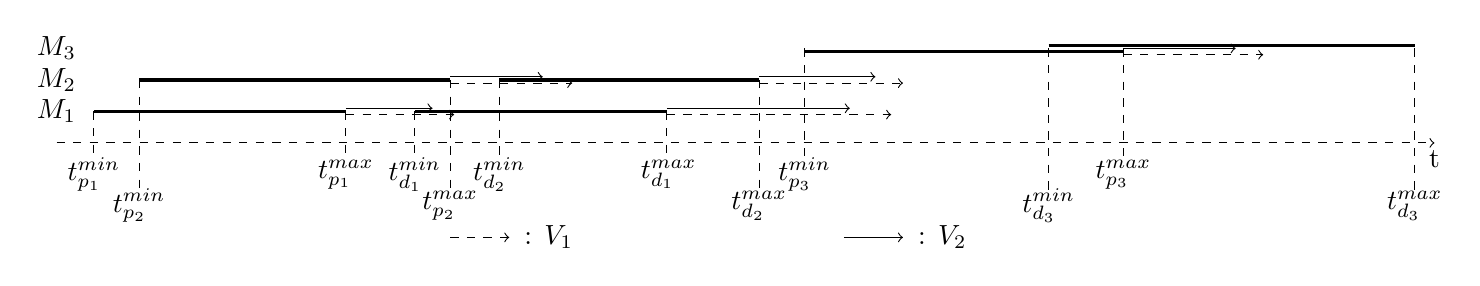
\begin{tikzpicture}[-,thick,xscale=0.25,yscale=0.4]
    \tikzstyle{v1}=[thin,dashed,->]
    \tikzstyle{v2}=[thin,->]
    \tikzstyle{tw}=[very thick,-,black]
    \tikzstyle{time}=[thin,dashed,->]
    \tikzstyle{trait}=[thin,dashed]

    \node (M1) at (5,1) {$M_1$};
    \node (M2) at (5,2) {$M_2$};
    \node (M3) at (5,3) {$M_3$};
    
    %M1
    \draw[tw] (6.9,1) -- (19.7,1);
    \draw[tw] (23.2,1) -- (36.0,1);
    %M2
    \draw[tw] (9.2,2) -- (25,2);
    \draw[tw] (27.5,2) -- (40.7,2);
    %M3
    \draw[tw] (43,2.9) -- (59.2,2.9);
    \draw[tw] (55.4,3.1) -- (74.0,3.1);

    %M1 : P -> D
    \draw[v1] (19.7,0.9) -- (25.2,0.9);
    \draw[v2] (19.7,1.1) -- (24.1,1.1);
    %M1 -> M3
    \draw[v1] (36,0.9) -- (47.4,0.9);
    \draw[v2] (36,1.1) -- (45.3,1.1);
    %M2 : P -> D
    \draw[v1] (25,1.9) -- (31.2,1.9);
    \draw[v2] (25,2.1) -- (29.7,2.1);
    %M2 -> M3
    \draw[v1] (40.7,1.9) -- (48,1.9);
    \draw[v2] (40.7,2.1) -- (46.6,2.1);
    %M3 : P -> D
    \draw[v1] (59.2,2.8) -- (66.3,2.8);
    \draw[v2] (59.2,3.0) -- (64.9,3);
    
    \draw[time] (5,0) -- (75.0,0);

    \draw[trait] (6.9,1) -- (6.9,-0.5);
    \draw[trait] (19.7,1) -- (19.7,-0.5);
    \draw[trait] (23.2,1) -- (23.2,-0.5);
    \draw[trait] (36,1) -- (36,-0.5);
    
    \draw[trait] (9.2,2) -- (9.2,-1.5);
    \draw[trait] (25,2) -- (25,-1.5);
    \draw[trait] (27.5,2) -- (27.5,-0.5);
    \draw[trait] (40.7,2) -- (40.7,-1.5);

    \draw[trait] (43,3) -- (43,-0.5);
    \draw[trait] (59.2,3) -- (59.2,-0.5);
    \draw[trait] (55.4,3) -- (55.4,-1.5);
    \draw[trait] (74,3) -- (74,-1.5);

    \node (m1PMin) at (6.9,-1) {$t_{p_1}^{min}$};
    \node (m1PMax) at (19.7,-1) {$t_{p_1}^{max}$};
    \node (m1DMin) at (23.2,-1) {$t_{d_1}^{min}$};
    \node (m1DMax) at (36.1,-1) {$t_{d_1}^{max}$};
    
    \node (m2PMin) at (9.2,-2) {$t_{p_2}^{min}$};
    \node (m2PMax) at (25,-2) {$t_{p_2}^{max}$};
    \node (m2DMin) at (27.5,-1) {$t_{d_2}^{min}$};
    \node (m2DMax) at (40.7,-2) {$t_{d_2}^{max}$};

    \node (m3PMin) at (43,-1) {$t_{p_3}^{min}$};
    \node (m3PMax) at (59.2,-1) {$t_{p_3}^{max}$};
    \node (m3DMin) at (55.4,-2) {$t_{d_3}^{min}$};
    \node (m3DMax) at (74,-2) {$t_{d_3}^{max}$};

    \node (t) at (75,-0.5) {t};

    \draw[v1] (25,-3) -- (28, -3);
    \draw[v2] (45,-3) -- (48,-3);

    \node (v1Legend) at (30, -3) { : $ V_1$ };
    \node (v2Legend) at (50, -3) { : $ V_2$ };
  \end{tikzpicture}

\caption{Exemple d'un problème à 2 machines ($V_1$ et $V_2$) and 3 tâches ($M_1$, $M_2$ et $M_3$).}
\label{fig:exempleJSSP}
\end{center}

\end{changemargin}
\end{figure}

\subsubsection{Fonction d'évaluation}
L'objectif est d'ordonnancer les tâches sur les machines de façon à minimiser la valeur de la fonction d'évaluation. Cette fonction reprend les critères définis pour la modélisation sous forme de problème de tournées de véhicules. Ainsi, la distance totale parcourue par les véhicules ainsi que la somme des retards pondérés sont les deux critères principaux. Dans une moindre mesure, l'avance des véhicules lors de l'arrivée sur les points de collecte et de livraison est également prise en compte afin de guider plus efficacement l'algorithme de résolution dans la recherche de la solution optimale.

\paragraph{Distance et durée de parcours}

Pour chaque séquence de tâches ($J_i$, $J_j$) réalisées par une machine $M_k$, la distance couverte est égale à :
\begin{equation}
\text{distance}(\text{position}(O_1^i),\text{position}(O_2^i)) + \text{distance}(\text{position}(O_1^j),\text{position}(O_2^j)) 
\end{equation}
Si $J_i$ est la première tâche exécutée par la machine, alors la distance vaudra :
\begin{equation}
\text{distance}(\text{position}(\text{depot}),\text{position}(O_1^i)) 
\end{equation}

Si $J_j$ est la dernière tâche exécutée, alors une distance supplémentaire doit être ajoutée à la distance totale parcourue correspondant au retour du véhicule au dépôt : 
\begin{equation}
\text{distance}(\text{position}(O_2^j),\text{position}(\text{depot}))
\end{equation}

Comme les autres critères d'évaluation d'une solution sont des mesures de temporelles, il est nécessaire de convertir cette distance parcourue en durée de parcours. Cette durée est obtenue en prennant en compte à la fois la vitesse du véhicule qui a couvert la distance, et à la fois le temps d'attente lié au trafic sur ce parcours pour ce véhicule. La durée est ainsi calculée selon l'équation \ref{eq:distance} (voir p. \pageref{eq:distance}) également utilisée par la modélisation sous forme de tournées de véhicules.

La durée totale du parcours d'un chariot cavalier $M_k$ liée à la réalisation des $card(W_k)$ tâches de son plan de charge $W_k$ est définie par l'équation suivante où $\kappa$ définit le temps de pose et de dépose d'un conteneur et est supposé constant : 
\begin{equation}
D^k = D^k_{(\text{depot},1)} + \sum \limits_{i=2}^{\text{card}(W_k)} \left( D^k_{(i-1, i)} \right) + D^k_{\left(\text{card}\left(W_k\right), \text{depot}\right)} + 2\kappa
\end{equation}


\paragraph{Retard et Avance}

Le deuxième et le troisième critère sont liés aux fenêtres de temps associées aux opérations des tâches. Si une mission dépasse une ou ses deux fenêtres de temps, alors un retard est comptabilisé. En fonction du type d'opération concernée, le retard peut engendrer le paiement de pénalités aux clients du terminal. Le retard ainsi comptabilisé devra être pondéré afin de ne prendre en compte uniquement les retards ayant un impact négatif sur le terminal. On définit ainsi $T_{ij,O_1}$ le retard (\textit{Tardiness}) lié au dépassement de la fenêtre de temps de collecte du conteneur de la mission $M_j$ après avoir réalisé la mission $M_i$, et $T_{ij,O_2}$ le retard lié au dépassement de la fenêtre de livraison de cette même mission. $y_j$ et $z_j$ sont des variables binaires indiquant respectivement si le retard de collecte et de livraison doivent être pris en compte. Le retard total $T^k_{ij}$ correspondra à la somme des retards de collecte et de livraison (voir \ref{eq:retardJSSP}).

\begin{equation}
 \label{eq:retardPickupJSSP}
 T^k_{ij,O_1} = \max \left( 0 , (t^k_P - TW_{j,1}^{\max}) \cdot y_j \right)
\end{equation}

\begin{equation}
 \label{eq:retardDeliveryJSSP}
 T^k_{ij,O_2} = \max \left( 0 , (t^k_D - TW_{j,2}^{\max}) \cdot z_j \right)
\end{equation}

\begin{equation}
 \label{eq:retardJSSP}
 T^k_ij = T_{ij,O_1} + T_{ij,O_2}
\end{equation}

De la même façon, l'avance (\textit{earliness}) d'un chariot cavalier $M_k$ pour une mission $j$ après avoir réalisé la mission $i$ est définie par la somme de l'avance du chariot cavalier au point de collecte au point de livraison de $j$ : 
\begin{equation}
 \label{eq:earlinessPickupJSSP}
   E^{k}_{ij,O_1} = \max \left( 0 , TW_{j,1}^{\min} - t^k_P\right)
\end{equation}

\begin{equation}
 \label{eq:earlinessDeliveryJSSP}
   E^{k}_{ij,O_2} = \max \left( 0 , TW_{j,1}^{\min} - t^k_P\right)
\end{equation}

\begin{equation}
 \label{eq:earlinessJSSP}
   E^{k}_{ij} = E^{k}_{ij,O_1} + E^{k}_{ij,O_2}
\end{equation}
 
 La fonction globale d'évaluation est donc définie par l'équation suivante: 
 
 \begin{equation}
  \label{eq:costJSSP}
  c^k_{ij} = D^k_{ij} \cdot F_1 + T^k_{ij} \cdot F_2 + E^k_{ij} \cdot F_3
 \end{equation}

 Le critère de l'avance ne servant qu'à guider l'algorithme de résolution il peut être écarté de la fonction d'évaluation. Le problème d'atelier correspondant au problème d'ordonnancement et d'affectation des missions aux chariots cavaliers est alors définit par la notation de Graham (voir \ref{chap:art:sec:jssp:subsec:def:graham}, p. \pageref{chap:art:sec:jssp:subsec:def:graham}) suivante : ${ J|ST_{sd}, R_{sd}|\sum w_j.T_{j} , \sum distance(i)}$.
 
 \subsection{Conclusion}
 
 La modélisation sous forme de problème d'atelier reprend exactement les mêmes équations que la modélisation sous forme de tournées de véhicules. Les seules différences se situent dans la formulation du problème et dans le vocabulaire ainsi utilisé. La résolution de l'une ou l'autre modélisation sera la même et visera à minimiser la valeur de la fonction globale d'évaluation proposée dans l'équation \ref{eq:ordo:cvrp} (voir p. \pageref{eq:ordo:cvrp}).
 
 Dans les deux formulations, la dynamique influence les données du modèle et chaque événement se produisant conduira à vérifier la validité de la solution préalablement calculée. Si la solution est devenue inutilisable, une nouvelle solution devra être calculée.
 
\section{Méthodes de résolution}

L'objet de cette thèse est de développer une méthode d'optimisation permettant de proposer une solution approchée à un problème dynamique sous incertitude. L'objectif est de proposer une méthode de résolution basée sur les connaissances actuelles des caractéristiques du problème sans prendre en compte les événements futurs. En effet, il ne sera pas question ici d'essayer de prévoir la réalisation ou la non réalisation, ni même la probabilité de réalisation d'un événement, mais plutôt de réagir aux nouvelles caractéristiques afin de toujours proposer une solution réalisable.

Afin de mesurer la performance relative de notre algorithme, une méthode de résolution exacte du problème est également proposée et revêt la forme d'un algorithme de \textit{Branch and Bound}. Cependant, la complexité de ce problème rend inapplicable une telle méthode même avec des instance de taille raisonnable. Des méthodes approchées ont alors été élaborées et utilisent des heuristiques gloutonnes selon différentes politiques.
Nous proposons ainsi dans ce chapitre le détail de ces méthodes ainsi que le fonctionnement de nos algorithmes dynamiques. Deux versions sont ainsi élaborées. L'une propose une solution hors-ligne et itérative au problème et doit être exécuté lors de chaque nouvel événement. L'autre est une méthode continue dite en ligne (\textit{on-line}) qui permet de proposer une solution à tout moment.

\subsection{Méthode de résolution exacte} \label{chap:ordo:reso:BB}

La recherche de la solution optimale au problème comporte deux étapes. D'une part la recherche d'une solution valide, puis prouver qu'il n'existe pas de solution plus performante que celle-ci. Pour ce faire, il est nécessaire de parcourir l'espace de recherche. Toutefois, cet espace est immense et une recherche exhaustive des solutions est inapplicable.
Afin d'éviter de parcourir inutilement tout l'espace de recherche, une borne supérieure est utilisée. L'initialisation de cette borne est réalisée grâce à une méthode gloutonne, puis elle est mise-à-jour en fonction des nouvelles solutions trouvée. Cette borne correspond à la valeur de la fonction d'évaluation de la meilleure solution trouvée jusqu'alors. Elle indique ainsi que la solution optimale est au moins aussi performante que la meilleure solution trouvée jusque là.
Une fois la borne initialisée, un parcours exhaustifs de l'espace des solutions est réalisé. Chaque mission est insérée dans le plan de charge de chaque véhicule selon toutes les combinaisons possibles. Après chaque insertion d'une mission dans un plan de charge, le score de la solution partielle est évalué et s'il dépasse la borne supérieure alors le sous-arbre de recherche ne sera pas exploré. Ceci permet de couper des branches entières de l'arbre de recherche des solutions.

\subsubsection{Exemple}
La figure \ref{fig:arbreBB} montre la construction de l'arbre des solutions du problème à 2 machines et 3 missions de l'exemple de la figure \ref{fig:exempleJSSP} (voir p. \pageref{fig:exempleJSSP}).


Dans cet exemple, les hypothèses les plus favorables sont considérées :
\begin{itemize}
 \item il n'y a pas de temps d'attente sur le réseau routier du terminal ($attente^k_{ij}(t)=0s$) ;
 \item les véhicules des clients sont sur place dès le début de la fenêtre de temps ;
 \item tous les retards impliquent des pénalités ($y_i=z_i=1$, $\forall i \in [1;n]$);
 \item les temps de pose et de dépose des conteneurs sont considérés nuls ($\kappa = 0s$) ;
 \item les véhicules sont stationnés au dépôt au moment de l'exécution de la première mission ;
 \item tous les véhicules sont disponibles;
 \item $F_1 = 1$, $F_2 = 10$ et $F_3 = 2$.
\end{itemize}

L'arbre de la figure \ref{fig:arbreBB}\subref{subfig:arbreBBinit} est construit par un processus de retour sur trace (\textit{backtracking}) permettant de générer toutes les combinaisons possible, sans toutefois gérer les doublons. Lors de l'évaluation, les branches de l'arbre ayant déjà été évaluées (doublons) seront coupées. 

Il est intéressant de noter que malgré la trivialité de cet exemple, il existe déjà 24 combinaisons possibles d'ordonnancement et d'affectation des missions aux chariots cavaliers.

La figure \ref{fig:arbreBB}\subref{subfig:arbreBBinitBorne} décrit l'initialisation de la borne supérieure réalisé en affectant toutes les missions au premier véhicule. En prennant en compte les hypothèses précédente, la branche $\{M_1,M_2,M_3\}\{\emptyset\}$ de l'arbre est construite et permet d'initialiser la borne à 1829. Le calcul des chemins se poursuit donc avec cette borne jusqu'à trouver une nouvelle borne supérieure (voir \ref{fig:arbreBB}\subref{subfig:arbreBBrech}) : ici 1211. Les calculs se poursuivent et la borne supérieure de 1211 se trouve dépassée lors du calcul du sous-arbre $\{M2,M1\} \{\emptyset\}$ dont le score est de 2084. Les sous-branches de cette partie de l'arbre sont donc élaguées (voir \ref{fig:arbreBB}\subref{subfig:arbreBBcoupure}). La recherche de borne supérieure est poursuivie jusqu'à ce que toutes les branches de l'arbre aient été soit évaluées soit élaguées. La solution optimale est donc : $\{M_2,M_3\}\{M_1\}$, dont le score de 1186 est indiqué sur le sous arbre rouge (voir \
ref{fig:arbreBB}\subref{subfig:arbreBBfinal}).

\input{chapitres/ordo/exempleBB}

Dans l'exemple précédent, la première borne trouvée est relativement fine. Néanmoins, elle aurait pu être bien plus large et par conséquent requérir l'exploration d'un nombre supérieur de sous-arbres. Une initialisation fine de la borne supérieure peut donc influencer positivement la performance de l'algorithme (vitesse de convergence). D'autre part, l'arbre de cet exemple est parcouru en profondeur dans l'ordre préfixe. L'évaluation est donc réalisée dès le premier sommet (racine $\rightarrow \{M1\}\{\emptyset\}$), ce qui permet d'arrêter l'évaluation d'une branche dont la partie supérieure dépasse la borne courante.  

\FloatBarrier

\subsubsection{Algorithmes}

L'algorithme \ref{algo:BranchAndBound} et la fonction \ref{algo:func:evaluationBranchAndBound} décrivent le fonctionnement de la méthode de séparation et évaluation. Cette méthode de résolution utilise l'arbre des solutions construit par un mécanisme de retour sur trace exhaustif (\textit{backtracking}). La seconde étape est l'évaluation de la borne supérieure initiale et est réalisée grâce à une des heuristiques présentées dans la section suivante (voir \ref{chapitre:ordo:sec:resolution:subsection:heuristiques} p.\pageref{chapitre:ordo:sec:resolution:subsection:heuristiques}). Une fois l'initialisation terminée, l'évaluation des sous-arbres débute par la racine de l'arbre. La fonction \textit{evaluation(A,S)} consiste donc à évaluer les fils de la racine de l'arbre $A$. Si un fils possède un score supérieur à la borne courante, sa branche est éliminée. Dans le cas contraire, la descente se poursuit récursivement dans son sous-arbre. Si le fils est une feuille et que son score est inférieur à la borne 
supérieure courante, alors cela signifie qu'il constitue une nouvelle borne. Une fois que tous les fils de la racine de l'arbre ont été évalués, la fonction d'évaluation renvoie le chemin qui relie la racine à une feuille et qui possède le score optimal.

Le processus de \textit{backtracking} générant plusieurs fois les même combinaisons, il est nécessaire de maintenir une structure de mémorisation des solutions déjà évaluées. Ainsi, lors de l'évaluation d'un fils, si celui-ci a déjà été évalué, il est éliminé. Sinon il est ajouté à la mémoire et il est évalué.

Il est possible de paralléliser les appels à la fonction d'évaluation à condition de synchroniser les accès à la borne supérieure ainsi qu'à la mémoire.

%TODO paragraphe sur les temps de calculs?

\begin{algorithm}[H]
\Res{Feuille de l'arbre ayant le score le plus faible}
\Deb{
$A \leftarrow$ initialiserArbre()\;
$S \leftarrow$ initialiserBorne($A$)\;
$S \leftarrow $ evaluation($A$,$S$)\;
\Retour{$S$\;}
}
\caption{Algorithme d'évaluation séparation}
\label{algo:BranchAndBound}
\end{algorithm}

\begin{function}[H]
\Donnees{\\
\begin{tabular}{m{0.2cm}m{0.1cm}m{13cm}}
  $A$ & : & sous-arbre à évaluer\\
  $S$ &: & borne supérieure courante
\end{tabular}
}
\Deb{
\PourCh{fils $f$ de $A$}{
  $fScore \leftarrow$ score($f$)\;
  \Si{$fScore \leq$ score($S$)}{
    \eSi{$f$ est une feuille}
      {
	%Nouveau record
	$S \leftarrow f$\;
      }
      {
	%On continu avec ses fils
	$S \leftarrow$ evaluation($f$,$S$)\;
      }
  }
  %Sinon on s'arrete
}
\Retour{$S$}
}
\caption{evaluation($A$,$S$)}
\label{algo:func:evaluationBranchAndBound}
\end{function}

\subsection{Méthodes de résolution approchées}\label{chapitre:ordo:sec:resolution:subsection:heuristiques}

Les méthodes de résolution approchées permettent de trouver rapidement une solution en sacrifiant la garantie d'optimalité de cette dernière. La qualité de la solution ainsi trouvée dépendra fortement de la stratégie utilisée pour son élaboration. Les principales stratégies utilisées sont la méthode des plus proches voisins, la méthode aléatoire et la méthode de répartition de charge. Enfin une méthode, basée sur la méthode gloutonne a été développée afin d'améliorer la qualité de la solution de cette dernière tout en modérant le temps de calcul.

%Méthode aléatoire
\subsubsection{Algorithme d'affectation aléatoire}\label{chap:ordo:reso:random}

Cette méthode consiste à déterminer les plans de charge des véhicules de façon aléatoire. À chaque étape une mission est tirée au sort, puis un véhicule est également choisi aléatoirement. La mission est insérée à la fin du plan de charge du véhicule choisi. Le processus est répété jusqu'à ce que toutes les missions aient été affectées.

Il est clair qu'aucune évaluation ne guide le choix des missions et des véhicules, ni concernant l'affectation, ni vis-à-vis de l'ordre de l'ajout des missions dans les plans de charge. L'inconvénient de cette méthode est donc de bien souvent produire des solutions de piètre qualité. En revanche, l'absence de calculs conduit une grande rapidité d'obtention d'une solution.

Vu la rapidité d'obtention d'une solution grâce à cette méthode, il est envisageable d'améliorer la qualité de la solution produite. Il est ainsi possible, par exemple, de combiner cette méthode avec l'heuristique \textit{2-opt} de Lin et Kernighan (voir \cite{Lin1973}), ou dans le cas général \textit{k-opt}, ou encore de produire plusieurs solutions et de ne conserver que la meilleure.

%Linear
\subsubsection{Politique de répartition de charge}\label{chap:ordo:reso:linear}

Cette méthode consiste à répartir les tâches sur les différentes ressources. Ainsi, les missions sont triées par date de début au plus tard, puis tour-à-tour affectées à un chariot cavalier différent. Lorsque tous les véhicules ont obtenu une mission, l'opération est répétée jusqu'à ce que toutes les missions aient été affectées.

Cette méthode permet d'éviter de dépasser les fenêtres de temps des missions en répartissant les missions proches temporellement sur différents chariots cavaliers. En revanche, elle provoque une augmentation de la distance parcourue car un grand nombre de véhicules sont utilisés et donc doivent rentrer au dépôt à la fin de leur tournée, alors que les trajets vers le dépôt sont minimisé en enchaînant plusieurs missions sur un même véhicule.

Au niveau de la complexité, cette méthode utilise un tri qui sera l'élément critique de performance de l'algorithme. Plus le tri sera efficace, plus la solution sera obtenue rapidement. De façon générale, les solutions sont obtenues très rapidement et sont de meilleure qualité que celles produites par la méthode aléatoire. Il est également possible de combiner cette méthode avec l'heuristique \textit{k-opt} ou d'utiliser de l'aléatoire dans le choix de l'ordre des véhicules, ou de combiner cette dernière méthode afin de générer plusieurs solutions et de ne garder que la plus performante.

%Greedy algorithm statique
\subsubsection{Algorithme glouton : méthode des plus proches voisins}\label{chap:ordo:sec:resolution:subsec:heuristiques:glouton}

La méthode des plus proches voisins consiste à déterminer les enchaînements de missions dont les coûts sont les plus faibles. Les couples (ressource,tâche) sont triés par coût, puis le couple de poids minimal est choisi. L'affectation se poursuit jusqu'à ce que toutes les missions aient été attribuées. Ici, la notion de proximité correspond donc, non pas à la distance entre les missions, mais bien à la valeur de la fonction d'évaluation associées à l'enchaînement des missions.

Cette méthode gloutonne permet d'obtenir rapidement des solutions sans garantie d'optimalité. Il s'agit d'une optimisation locale liée à chaque nouvelle affectation de mission. L'optimisation globale résultant de la somme des optimisations locales est bien souvent de mauvaise qualité. La méthode développée dans le paragraphe suivant permet d'améliorer la qualité de la solution obtenue par la méthode des plus proches voisins.

%Greedy algorithm dynamique
\subsubsection{Méthode gloutonne élaborée}\label{chap:ordo:reso:greedyOpt}

Cette heuristique consiste à déterminer pour chaque mission à affecter, à la fois le véhicule à associer ainsi que la position d'insertion de la mission dans le plan de charge du véhicule, de façon à minimiser la valeur de la fonction d'évaluation. Ainsi, pour chaque mission, toutes les combinaisons possibles d'insertion sont calculées et la mission est insérée dans le plan de charge du véhicule et à l'indice de coût minimal.
Il s'agit également d'optimisation locale car le résultat dépend de l'ordre dans lequel les missions sont considérées, mais qui fournit des solutions de meilleure qualité que la simple méthode des plus proches voisins.
Toutefois, le temps de calcul d'un tel ordonnancement est bien supérieur à celui des méthodes heuristiques évoquées précédemment du fait du nombre de combinaisons à tester.
Elle ne sera donc pas utilisable pour des instances de grande taille.


\subsection{Méthodes dynamiques}

Les méthodes heuristiques permettent d'obtenir une solution au problème en privilégiant la rapidité de calcul à la qualité. La complexité du problème, même dans le cas statique, rend inapplicable une approche de résolution exacte. Dans le cas dynamique il sera nécessaire de recalculer la solution à chaque changement d'une caractéristique du problème. Les méthodes de résolution doivent donc être en mesure de calculer une solution suffisamment rapidement pour rester valide au moment de son application. Parallèlement au besoin de réactivité, la méthode de résolution doit fournir une solution dont la qualité est proche de la solution optimale.

Pour toutes ces raisons, cette thèse introduit une méthode de résolution dynamique basée sur une métaheuristique. Une méthode à base de colonies de fourmis est utilisée pour produire l'ordonnancement et l'affectation de missions aux chariots cavaliers. Deux versions de l'algorithme ont été mises au point : l'une permettant d'obtenir une solution de façon itérative et l'autre de façon continue.

La première méthode est dite hors-ligne (\textit{off-line}) et permet de calculer une solution dès qu'une caractéristique du problème a changé. La solution ainsi obtenue est complète. La seconde méthode, est une méthode en ligne (\textit{on-line}) permettant de calculer continuellement une solution au problème. Cette solution peut ici être partielle et les missions non-affectées à l'instant $t$ le seront à l'instant $t+t'$.

%Algorithme fourmis itératif (avec graphe complet)
\subsubsection{Méthode de résolution hors-ligne à colonies de fourmis}\label{chap:ordo:reso:offlineACO}

Cette méthode résout de façon dynamique le problème de voyageurs de commerce associé au problème d'ordonnancement et d'affectation de missions. La métaheuristique reprend le comportement naturel des individus d'une colonie de fourmis. Ici, chaque fourmi artificielle de la colonie représente un voyageur de commerce, c'est-à-dire un chariot cavalier. Il y a donc $m$ fourmis dans la colonie qui évolue sur un graphe.

\paragraph{Graphe}

Soit le graphe complet $G^{(t)}=(V,A)$ où :

\begin{itemize}
 \item $V$ est l'ensemble des sommets et est constitué des villes à visiter (missions à réaliser) $v_1 \cdots v_n$ plus le sommet représentant le dépôt des véhicules $v_0$;
 \item $A$ est l'ensemble des arcs $(v_i,v_j)$ indiquant la visite de la ville $v_j$ immédiatement après $v_i$.
\end{itemize}

La section \ref{chapitre:ordo:sec:modelisation:subsec:vrp} (voir p. \pageref{chapitre:ordo:sec:modelisation:subsec:vrp}) décrit la construction d'un tel graphe.

Chaque fourmi artificielle est initialisée sur le noeud de dépôt et l'algorithme prend en compte : 
\begin{itemize}
 \item soit la position courante du chariot cavalier correspondant s'il est inactif au moment du calcul de la solution;
 \item soit la position future du véhicule ainsi que sa date de disponibilité s'il est occupé.
\end{itemize}

\paragraph{Gestion de la phéromone}

L'algorithme proposé fonctionne sur un mécanisme de collaboration/compétition entre les fourmis. L'objectif pour une fourmi est de lutter contre les autres fourmis afin de coloniser des missions à réaliser pour le chariot cavalier correspondant. Il s'agit de l'objectif local. Au niveau de la colonie, l'objectif est de répartir les missions de façon ordonnée sur les différentes fourmis afin de minimiser une fonction d'évaluation.
Pour ce faire, chaque fourmi possède sa propre marque de phéromone. Ainsi la quantité de phéromone de la fourmi $k$ sur l'arc $(v_i,v_j)$ au temps $t$ est noté $\tau^k_{ij}(t)$. La quantité de phéromone des autres fourmis est noté $\hat \tau^k_{ij}(t)$.

\begin{equation}
  \hat \tau^k_{ij}(t) = \left( \sum \limits_{l=1, l \neq k}^{m} (\tau^l_{ij}(t)) \right)
\end{equation}

Grâce à cette distinction des traces de phéromone, il est possible pour une fourmi d'être attirée par les chemins comportant sa phéromone, et repoussée par ceux comportant des traces de phéromone étrangère.

\subparagraph{Renforcement des pistes\\}

Lorsque toutes les missions ont été colonisées par les fourmis, la solution ainsi créée est évaluée. Une politique de marquage de type élitiste est alors réalisée, c'est-à-dire que seuls les chemins de la meilleure solution sont marqués en phéromone par les fourmis. Les chemins des autres solutions sont ainsi ``oubliés'' par la colonie ce qui permet de minimiser le bruit créé par ces solutions au cours de la recherche. Ainsi $\Delta^k_{ij}(t)$ indique la quantité de phéromone déposée par la fourmi $k$ sur l'arc $(v_i,v_j)$ au temps $t$ et est définit par l'équation suivante :

\begin{equation}\label{eq:acoIteratif:renforcement}
 \Delta^k_{ij}(t) = 
 \begin{cases}
    \frac{1}{c^k_{ij}(t)} & \text{ si le score du chemin à marquer est un nouveau record}\\
    0 & \text{ sinon}
 \end{cases}
\end{equation}

\subparagraph{Évaporation\\}

Afin d'empêcher l'algorithme de rester piégé dans une solution localement optimale, les traces de phéromone sont continuellement évaporées. Cette évaporation est réalisée après chaque solution calculée. Le paramètre $\rho$ ($\rho \in [0;1]$) permet de définir le taux de conservation de la phéromone. Quand $\rho = 1$, il n'y a pas d'évaporation.

La quantité de phéromone de la fourmi $k$ présente au temps $t$ sur un arc $(v_i,v_j)$ est définie par l'équation \ref{eq:acoIteratifPheromone}. Cette quantité est bornée dans l'intervalle $\left[\lambda ; +\infty\right[$ afin de garantir la présence de phéromone sur chaque arc à tout moment.

\begin{equation}\label{eq:acoIteratifPheromone}
 \tau^k_{ij}(t) = \max \left(\lambda , \rho \cdot \tau^k_{ij}(t-1) \right) + \Delta^k_{ij}(t)
\end{equation}

\paragraph{Comportement des fourmis}

Une fourmi se déplace sur le graphe $G$ grâce à la règle de transition décrite dans le paragraphe suivant. À chaque fois qu'une fourmi $k$, présente sur le noeud $i$, doit choisir une destination, les probabilités de choix des destinations possibles ($p^k_{ij}$) sont calculées. Un tirage au sort proportionnel détermine alors la destination choisie. 

À chaque déplacement d'une fourmi sur le graphe, le coût du chemin courant est évalué et le sommet choisi est rendu inaccessible pour les autres fourmis. On peut ainsi remarquer que c'est ce procédé de gestion des sommets à l'échelle globale qui permet d'obtenir une solution complète c'est-à-dire une solution dont les chemins contiennent toutes les missions à réaliser. En revanche, cette gestion globale est contraire au fonctionnement traditionnel des algorithmes fourmis dont la caractéristique principale repose sur le comportement totalement décentralisé des fourmis.

Lorsque plus aucun déplacement n'est possible, c'est-à-dire que toutes les villes ont été visitées, les fourmis sont replacées à leur position initiale sur le graphe et la solution est évaluée. La fonction d'évaluation du chemin global prend en compte les fonctions d'évaluation du chemin de chaque fourmi. Toutefois, les paramètres $F_1$, $F_2$ et $F_3$ servant à guider la recherche locale, il peut être utile d'utiliser des valeurs différentes lors de l'évaluation de la solution globale. Pour cette raison, l'évaluation de l'enchaînement total des missions par les chariots cavaliers $c(t)$ est calculée ainsi par l'équation suivante : 

\begin{equation}
 c(t) = \sum \limits_{i=0}^n \sum \limits_{j=0, j\neq i}^n \sum \limits_{k=1}^m \left(c'^k_{ij}(t) \cdot x^k_{ij}(t)\right) 
\end{equation}

Où $c'^k_{ij}(t)$ se définit comme tel :
\begin{equation}
 c'^k_{ij}(t) = d^k_{ij}(t) \cdot F_1' + l^k_{ij}(t) \cdot F_2' + e^k_{ij}(t) \cdot F_3'
\end{equation}

Dans le cas où le chemin ainsi construit obtient un meilleur score que le meilleur chemin trouvé jusqu'alors, la phéromone est déposée. Sinon aucune phéromone n'est déposée par les fourmis. L'évaporation est réalisée à chaque fois qu'une nouvelle solution a été obtenue par les fourmis.

\subparagraph{Règle de transition pseudo-aléatoire proportionnelle\\}

Une fourmi choisit aléatoirement une mission à réaliser parmi les missions non-affectées selon les probabilités calculées par l'équation \ref{eq:acoIteratif:transition} : 

\begin{equation} \label{eq:acoIteratif:transition}
 p^k_{ij}(t) = \frac{\bigg[\tau^k_{ij}(t)\bigg]^\alpha \cdot \bigg[1 + \frac{1}{c^k_{ij}(t)}\bigg]^\beta \cdot \bigg[1 + \frac{\tau^k_{ij}(t)}{\sum \limits_{l=1}^{m} \tau^l_{ij}(t)}\bigg]^\gamma}
 {\sum \limits_{s \in S_i} \left(\bigg[\tau^k_{is}(t)\bigg]^\alpha \cdot \bigg[1 + \frac{1}{c^k_{is}(t)}\bigg]^\beta \cdot \bigg[1 + \frac{\tau^k_{is}(t)}{\sum \limits_{l=1}^{m} \tau^l_{is}(t)}\bigg]^\gamma\right)}
\end{equation}

Cette règle de transition pseudo-aléatoire proportionnelle indique la probabilité pour qu'un voyageur $k$ choisisse la ville $j$ immédiatement après avoir visité la ville $i$ au temps $t$ (et donc parmi les successeurs $s$ de $i$ ($s \in S_i$)). Cette règle prend en compte trois facteurs :

\begin{tabular}[\textwidth]{m{2.5cm} m{0.2cm} m{11.5cm}}
 $\Big[\tau^k_{ij}(t)\Big]$ & : & la quantité de phéromone de la fourmi $k$ présente sur l'arc $(v_i,vj)$; \\
 $\Big[1 + \frac{1}{c^k_{ij}(t)}\Big]$ & : & l'inverse du coût d'enchaînement de la visite de la ville $j$ après la ville $i$ pour le voyageur $k$ au temps $t$;\\%\rule[0pt]{0pt}{40pt} \\
 $\Big[1 + \frac{\tau^k_{ij}(t)}{\sum \limits_{l=1}^{m} \tau^l_{ij}(t)}\Big]$ & : & la part de phéromone de la fourmi $k$ sur l'arc $(v_i,v_j)$ au temps $t$.
\end{tabular}\\

Le premier terme de l'équation (quantité de phéromone de la fourmi $k$ sur l'arc $(v_i,v_j)$) permet d'indiquer la qualité de l'insertion de l'arc dans la solution construite. Plus la qualité de la solution précédemment construite est importante et plus la quantité de phéromone déposée sur les arcs sera élevée (voir équation \ref{eq:acoIteratif:renforcement} p.\pageref{eq:acoIteratif:renforcement}). Ce terme permet aux fourmis de communiquer les unes avec les autres. Cette stigmergie modélise également une forme de mémoire en permettant aux fourmis d'accéder à une connaissance de l'évaluation passée de la qualité d'une section de chemin. De part cette communication, les fourmis vont être en mesure de collaborer les unes avec les autres.

La fonction de coût est décrite par l'équation \ref{eq:cost} (voir p.\pageref{eq:cost}) et prend en compte la durée de déplacement des voyageurs, le retard pondéré ainsi que l'avance. C'est la partie heuristique de l'équation. Elle permet de guider la recherche vers des optimums locaux et ainsi d'accélérer la vitesse de convergence de l'algorithme. Mis à part de l'emploi de l'aléatoire ainsi que de l'utilisation de la phéromone, cette partie de la formule correspond à l'heuristique des plus proches voisins (voir \ref{chap:ordo:sec:resolution:subsec:heuristiques:glouton} p.\pageref{chap:ordo:sec:resolution:subsec:heuristiques:glouton}).

Le troisième et dernier terme : $\bigg[1 +\frac{\tau^k_{ij}(t)}{\sum \limits_{l=1}^{m} \tau^l_{ij}(t)}\bigg]$ n'est pas présent dans la loi de transition traditionnelle d'un ACO (voir \ref{eq:as:transition} p.\pageref{eq:as:transition}). Il introduit un processus de compétition entre les fourmis. Ainsi, plus il y aura de phéromone étrangère sur un arc et plus la fourmi sera repoussée. En revanche si la part de phéromone de la fourmi est importante alors elle sera attirée par cet arc.

Les constantes $\alpha$, $\beta$, et $\gamma$ ($0 \leq \alpha,\beta, \gamma < + \infty$) permettent de pondérer l'importance relative des trois termes de la formule. 
L'inverse du coût de l'enchaînement de deux missions ainsi que la part de phéromone de la fourmi sur la phéromone totale présente sur l'arc sont bornés sur $\left]0;1\right]$. Leur valeur est donc augmentée afin d'être comprise sur $\left[1;2\right]$ afin que l'application de la puissance $\beta$ et $\gamma$ donne un résultat sur l'intervalle $\left]1;+\infty\right[$. 
Le dénominateur de l'équation permet ensuite d'obtenir un résultat compris dans l'intervalle $[0;1]$.

\paragraph{Algorithme général}

L'algorithme principal (voir Algorithme \ref{algo:acoIteratif}) prend en paramètre la liste des véhicules ainsi et que le graphe des missions à ordonnancer et à affecter. À chaque itération de l'algorithme, un véhicule est tiré au sort se déplace en fonction de la loi de transition \ref{eq:acoIteratif:transition} jusqu'à ce que toutes les missions aient été attribuées. Ensuite, les scores des plans de charge ainsi déterminés sont additionnés pour obtenir le score total de l'ordonnancement. Si ce score est le meilleur obtenu jusqu'à présent, il est sauvegardé et les fourmis déposent de la phéromone sur leurs chemins respectifs. Enfin la phéromone est évaporée et le processus est réitéré pendant $\Theta$ itérations.

\begin{algorithm}
\Res{\\\vspace{-7pt}
\begin{tabular}{l}
Plan de charge des machines
\end{tabular}
}
\Donnees{\\
\begin{tabular}{l}
 M : liste des véhicules,\\
 V : sommets du graphe,\\
 A : arcs du graphe
\end{tabular}} 
\Deb{
$meilleurScore \leftarrow +\infty$\;
$meilleurChemin \leftarrow \emptyset$\;
$etape \leftarrow 1$\;
\Tq{$etape \leq \Theta$}{
  $P \leftarrow N$\;
  $chemins \leftarrow \emptyset$\;
  \PourCh{fourmi $k$ de $M$}{
    $initialiserPosition()$\;
    $chemin^k \leftarrow \emptyset$\;
    $chemins \leftarrow chemin^k$\;
  }
  \Tq{$P \neq \emptyset$}{
    $k = alea(M)$\;
    $j = choisirDestination(k,P)$\;
    $chemin^k \leftarrow j$\;
    $P \leftarrow P - {j}$\;
  }
  $score \leftarrow sommeScore(chemins)$\;
  \Si{$score < meilleurScore$}{
    $meilleurScore \leftarrow score$\;
    $deposerPheromone(chemins)$\;
  }
  $evaporation(N)$\;
  $etape \leftarrow etape + 1$\;
} %FTq
\Retour{$meilleurChemin$\;}
}
\caption{méthode de résolution dynamique hors-ligne}
\label{algo:acoIteratif}
\end{algorithm}

\paragraph{Gestion de la dynamique}

Cette méthode de résolution du problème est dite hors-ligne car elle doit être exécutée à chaque fois qu'une caractéristique du problème change. Chaque événement survenant sur le terminal modifie les données du problème et une solution calculée au temps $t$ peut ne plus être valable au temps $t'$. Ainsi, les entrées de l'algorithme sont modifiés à chaque nouvelle exécution.

En revanche, même si les coûts des arcs ou les sommets du graphe, ou encore le nombre ou les caractéristiques des véhicules changent, les traces de phéromone présentes sur les arcs du graphe sont conservées. Cette conservation permettra de guider les fourmis dans leur nouvelle recherche de solution. En effet, malgré les modifications des caractéristiques du problème, une partie de la solution précédemment calculée peut rester valide.

C'est ce mécanisme de conservation de phéromone qui rend la métaheuristique fourmi adaptée à la résolution de problèmes dynamiques.

\paragraph{Paramètres}

Le défaut majeur de la métaheuristique fourmi réside dans le nombre important de paramètre ainsi que dans l'incidence de leur valeur vis-à-vis de la qualité de la solution trouvée et de sa vitesse d'obtention. La méthode de résolution hors-ligne utilise les paramètres suivants : 

\begin{tabular}{ccp{0.9\textwidth}}
 $\alpha$ &:& importance relative de la trace de phéromone lors du choix de la destination;\\
 $\beta$ &:& importance relative de l'heuristique de pondération lors du choix de la destination;\\
 $\gamma$ &:& importance relative du processus de répulsion lors du choix de la destination;\\
 $\lambda$ &:& quantité minimale de phéromone présente sur chaque arc;\\
 $\rho$ &:& taux de conservation de la phéromone après chaque itération de l'algorithme;\\
 $F_1$ &:& importance relative de la durée des trajets dans l'évaluation de l'enchaînement de deux missions;\\
 $F_2$ &:& importance relative du retard pondéré dans l'évaluation de l'enchaînement de deux missions;\\
 $F_3$ &:& importance relative de l'avance dans l'évaluation de l'enchaînement de deux missions;\\
 $F_1'$ &:& importance relative de la durée des trajets dans l'évaluation globale d'une solution;\\
 $F_2'$ &:& importance relative du retard pondéré dans l'évaluation globale d'une solution;\\
 $F_3'$ &:& importance relative de l'avance dans l'évaluation globale d'une solution;\\
 $\Theta$ &:& nombre d'itérations de la boucle principale de l'algorithme à effectuer à chaque exécution.
\end{tabular}

La valeur idéale pour chacun de ses paramètres se détermine de manière empirique. Néanmoins, il est possible de prédéfinir des valeurs initiales en prennant en compte les relations mathématiques entre ces paramètres.\\

Le paramètre $\Theta$ permet de contrôler le rapport entre la qualité de la solution et la durée du calcul. Un $\Theta$ important conduira à de meilleures solutions mais également à des calculs plus longs. Il peut-être nécessaire de réduire la valeur de $\Theta$ dans le cas où la dynamique du système est trop importante et provoque des modifications sur les caractéristiques du problème avant que l'algorithme ait le temps de proposer une solution. Pour cela il peut être utile de connaître le temps de calcul d'une itération et d'utiliser les connaissances sur la dynamicité du système (statistiques, degré effectif de dynamicité, etc.) afin de déterminer le nombre d'itérations optimal. Ce temps de calcul d'une itération dépendra, mis à part des performances de la machine utilisée pour le calcul, de la taille du problème, c'est-à-dire du nombre de missions à ordonnancer ainsi que du nombre de véhicules à utiliser.\\

Le calcul du temps moyen de trajet par mission permet d'initialiser les paramètres $F_1$, $F_2$ et $F_3$. En effet, ces paramètres contrôlant une importance relative, il est nécessaire d'évaluer les parts de retard et d'avance tolérées par mission afin de les initialiser. Par exemple, si la durée moyenne du déplacement d'une mission est de 2 minutes et qu'on tolère 30 seconde de retard et 6 minutes d'avance par mission, on pourra définir : 
\begin{itemize}
 \item $F_1 = 4$ ($2$ minutes = $4 * 30$ secondes)
 \item $F_2 = 1$ 
 \item $F_3 = 12$ ($6$ minutes = $12 * 30$ secondes)
\end{itemize}

Ces paramètres étant pris en compte dans l'évaluation heuristique du poids d'un arc, ils sont utilisés dans la règle de transition proportionnelle et cette valeur est pondérée par le paramètre $\beta$. Une mission consistant à déplacer un conteneur, le temps de réalisation ne peut être nul. Dans l'hypothèse d'une discrétisation à la seconde, la valeur de la partie droite du deuxième terme de la loi de transition est comprise entre 0 et 1. Puis la valeur est incrémentée afin d'appartenir à l'intervalle $\left[1;2\right]$. Mis à la puissance $\beta$, le résultat est définit sur $\left[1;+\infty\right]$.\\

La partie droite du dernier terme de la règle de transition étant un ratio, il est compris entre 0 et 1. Là encore, la valeur est incrémentée pour être définie sur $\left[1;2\right]$, puis sur $\left[1;+\infty\right]$ après la mise à la puissance $\gamma$.\\

Le paramètre $\lambda$ doit être définit sur $\left[1;+\infty\right]$ afin d'assurer que le premier terme de la règle de transition puisse être définit sur $\left[1;\infty\right[$.\\

Le paramètre $\rho$ représente la part de phéromone conservée après chaque évaporation et se définit sur $\left[0;1\right]$. Pour une même valeur de $\rho$, plus la trace de phéromone présente sur un arc sera importante et plus la quantité évaporée sera grande. L'utilisation d'un fort taux d'évaporation combiné à une faible présence de phéromone conduira à l'inefficacité du système de communication entre les fourmis. Au contraire, une évaporation faible alliée à une présence forte de phéromone provoquera l'inefficacité du processus d'évaporation et les arcs seront saturés de phéromones. La conséquence sera que les anciennes meilleures solutions, devenues invalides avec le temps, continueront d'attirer les fourmis, au détriment de nouvelles solutions potentielles.\\

Toutes ces valeurs conditionnent grandement l'efficacité de l'algorithme et leur définition requiert de nombreux ajustement du fait des interactions entre les paramètres. Ils constituent le point faible de la métaheuristique fourmi en général, et ici de la méthode fourmi appliquée au problème d'ordonnancement et d'affectation.

%Algorithme fourmis continu (avec graphe élagué)
\subsubsection{Méthode de résolution en-ligne à colonies de fourmis}\label{chap:ordo:reso:onlineACO}

Cette méthode se rapproche de la méthode décrite dans le paragraphe précédent. Il est également question de métaheuristique fourmi ainsi que de phéromone colorée. Ici il y aura autant de colonies de fourmis qu'il y a de voyageurs dans le problème des voyageurs de commerce connexe. Ainsi, une colonie est modélisée par une couleur et chaque fourmi de la colonie dépose de la phéromone de la couleur de la colonie. Les fourmis d'une colonie sont attirées par les pistes contenant de la phéromone de leur couleur, et repoussées par les pistes contenant de la phéromone des autres couleurs. 

%\paragraph{Motivations}
Cet algorithme a été élaboré dans le but de proposer rapidement une solution au problème, peu importe son degré de dynamicité. Pour ce faire, il est nécessaire d'intégrer cette dynamicité dans le modèle même de la méthode de résolution, afin d'éviter de recalculer complètement une solution à partir de zéro.

La méthode hors-ligne décrite dans le paragraphe précédent étant déjà rapide et utilisant également la métaheuristique fourmi, la seule possibilité d'accélération de la résolution du problème réside dans la structure du graphe sur lequel évoluent les fourmis. 
Il ne sera pas question ici de modéliser toutes les solutions possibles. Le graphe ne sera donc pas complet et seules les solutions dont le coût est ``raisonnable'' seront envisagées. On parlera de tâches compatibles pour indiquer qu'une tâche peut être réalisée après une autre par la même ressource. Deux tâches seront ainsi compatibles si les fenêtres de temps permettent théoriquement de réaliser les deux missions sans dépassement. %TODO : à une marge près ?

\paragraph{Description générale du graphe}

Définissons le graphe dynamique et orienté $G^{(t)}=(V,A)$ où $V$ est l'ensemble des n\oe{}uds et $A$ l'ensemble des arcs. Lors de l'initialisation, chaque tâche à ordonnancer (ou ville à visiter selon la modélisation) est modélisée par un n\oe{}ud $v_i \in V$ et les arcs $a_{ij} = (v_i,v_j) \in A$ représentent la possibilité pour les machines (ou les voyageurs de commerce) d'enchaîner la tâche $J_j$ (ou la ville $v_j$) après $J_i$ ($v_i$) sans dépasser les fenêtres de temps. Ainsi, un arc est ajouté entre deux n\oe{}uds $v_i$ et $v_j$ si pour au moins une ressource (voyageur) $k$, $TW_{i,2}^{\max} + setup^{k}_{ij} < TW_{j,1}^{\min}$. Au cours du processus de résolution, dès qu'une mission est réalisée par un chariot cavalier, le sommet correspondant est supprimé du graphe et la structure du graphe est corrigée comme décrit dans les paragraphes suivant afin de maintenir les propriétés du modèle.

En plus des tâches à planifier, deux sommets sont ajoutés au graphe : le noeud de source : $v_{source}$, et le noeud de fin : $v_{fin}$. Le noeud source est relié à chaque noeud du graphe dont le degré entrant est nul. Le degré entrant de $v_{source}$ est également nul. Les sommets du graphe dont le degré sortant est nul sont connectés au noeud $v_{fin}$, qui possède quant à lui uniquement des arcs entrant.

\paragraph{Colonies et véhicules}

Dans ce modèle, une colonie de fourmis représente un véhicule (machine ou voyageur selon la modélisation). Le véhicule doit choisir la meilleure séquence de missions à réaliser, c'est-à-dire celle qui minimise à la fois la distance parcourue, le retard pondéré et l'avance. Ainsi, les séquences de missions pour différents véhicules sont modélisées par des chemins distincts sur le graphe. 

Les fourmis d'une colonie doivent coloniser le graphe des missions de façon à trouver des chemins qui minimisent la valeur de la fonction d'évaluation.
Quand une fourmi atteint un sommet (correspondant à une mission), elle dépose de la phéromone sur celui-ci. Cette phéromone sera utilisée pour guider les autres fourmis de la colonie vers le n\oe{}ud et pour repousser les fourmis des autres colonies vers d'autres n\oe{}uds.
Comme chaque colonie agit de la même façon, les sommets sont répartis entre les différentes colonies et cette distribution tend à minimiser la fonction d'évaluation globale.

Chaque colonie est modélisée par une couleur. De cette façon, chaque n\oe{}ud du graphe est coloré par la couleur de la colonie dont la phéromone est la plus présente sur ce sommet. La solution globale est obtenue en construisant les meilleurs chemins pour chaque couleur. Chaque chemin $P^k$ de couleur $k$ est construit en partant de $v_{source}$. Lors de la construction du chemin, à partir d'un n\oe{}ud $v_i$ de couleur $k$, le prochain sommet est choisit parmi les successeurs de $v_i$ de couleur $k$ : $S^k_i$. Le n\oe{}ud choisit est celui comportant la plus grande quantité de phéromone de couleur $k$. Le processus est répété jusqu'à ce que $v_{fin}$ ait été atteint ou que $S^k_i=\emptyset$.

\paragraph{Pondération des arcs}

Un arc $a_{ij}$ relie le sommet $v_i$ à $v_j$ et correspond à l'enchaînement de la mission $j$ après la réalisation de la mission $i$. Cet arc est pondéré par le coût de l'enchaînement des deux missions sur la même machine. Ce poids doit prendre en compte à la fois la distance parcourue par le véhicule ainsi que le retard pondéré et l'avance engendrés par l'enchaînement des missions.

Les critères de la fonction d'évaluation sont les mêmes que pour le modèle hors-ligne de résolution dynamique. La distance correspond au temps de parcours entre le point de livraison du conteneur de la mission $i$ et le point de collecte du conteneur de la mission $j$ et est définie par l'équation \ref{eq:distance} (voir p. \pageref{eq:distance}). Le retard pondéré et l'avance sont décrits par les équations \ref{eq:tardiness2} et \ref{eq:earliness} (voir p. \pageref{eq:tardiness2}, et p. \pageref{eq:earliness}). Les variables $F_1$, $F_2$ et $F_3$ permettent de pondérer les critères les uns vis-à-vis des autres dans la fonction locale d'évaluation (voir eq. \ref{eq:cost} p. \pageref{eq:cost}).

La flotte de véhicules pouvant être hétérogène, chaque arc devra contenir autant de poids qu'il y a de machines (voyageurs) dans le problème puisque les temps de parcours diffèrent d'un véhicule à l'autre si leur vitesse est différente. 

Pour calculer les poids d'un arc, il est nécessaire de distinguer deux cas selon les extrémités de cet arc :
\begin{itemize}
 \item $v_j \neq v_{fin} $ : le poids de l'arc est donnée par l'équation précédente.
 \item $v_j = v_{fin}$ : le poids correspond uniquement au temps de parcours entre le point de livraison de la mission $j$ et le dépôt à la date de livraison prévue de la mission $j$;
\end{itemize}

\paragraph{Maintient de la structure du graphe}

Les sommets $v_{source}$ et $v_{fin}$ étant respectivement reliés uniquement aux sommets sans prédécesseur et sans successeur, il est nécessaire de modifier le graphe pour maintenir ces propriétés lors de l'ajout et de la suppression de sommets. 
Dans le cas décrit par la figure \ref{fig:suppressionSommet} où un sommet $v_i$ est l'unique prédécesseur de $v_j$ et où $v_{source}$ est relié à $v_i$ et $v_j$ est connecté à $v_{fin}$, lorsque la mission modélisée par le sommet $v_i$ sera exécutée par un véhicule, le sommet $v_i$ sera supprimé du graphe et un arc reliant $v_{source}$ à $v_j$ sera ajouté.
Dans la même situation où $v_j$ est le seul successeur de $v_i$, lorsque $v_j$ est réalisée par un véhicule, $v_j$ est supprimé du graphe et un arc reliant $v_i$ au sommet $v_{fin}$ est ajouté au graphe.
Lorsqu'un sommet $v_l$ est ajouté sur le graphe entre $v_{source}$ et $v_i$, $v_i$ possède alors deux successeurs  $v_{source}$ et $v_l$. L'arc $(v_{source},v_i)$ est alors supprimé et un arc est ajouté entre $v_{source}$ et $v_l$.
De la même façon, si $v_l$ devient le successeur de $v_j$ et que $v_j$ est le seul prédécesseur de $v_l$, alors l'arc $(v_j,v_{fin})$ est supprimé et un arc est ajouté entre $v_l$ et $v_{fin}$.

\begin{figure}[h]
\centering
\tiny
\tikzstyle{vertex}=[circle,draw,fill=white,line width=0.5pt,minimum size=25pt,inner sep=0pt,font=\tiny]
\tikzstyle{selected vertex} = [vertex]
\tikzstyle{red vertex} = [vertex, fill=black!100, text=white]
\tikzstyle{blue vertex} = [vertex, fill=black!40]
\tikzstyle{edge} = [draw,thick,->]
\tikzstyle{weight} = [font=\tiny]
\tikzstyle{weightRed} = [font=\tiny, black!100]
\tikzstyle{weightBlue} = [font=\tiny, black!40]
\tikzstyle{red edge} = [draw,thick,->,red!100]
\tikzstyle{blue edge} = [draw,thick,->,blue!100]
\tikzstyle{ignored edge} = [draw,line width=5pt,-,black!20]
 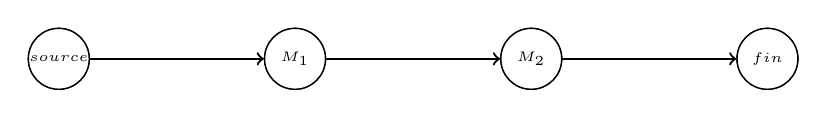
\begin{tikzpicture}[xscale=3, yscale=0.5, auto,swap]
 
    \foreach \pos/\name in {
	{(0,1)/source},
	{(1,1)/M_1}, {(2,1)/M_2},
	{(3,1)/fin}}
      \node[vertex] (\name) at \pos {$\name$};

    \foreach \source/ \dest in {source/M_1, M_1/M_2, M_2/fin} \path[edge] (\source) node[] {} -- node[] {} (\dest);
    
    \foreach \vertex in {source,M_1,M_2,fin}
        \path node[selected vertex] at (\vertex) {$\vertex$};
\end{tikzpicture}\\
Graphe initial\\

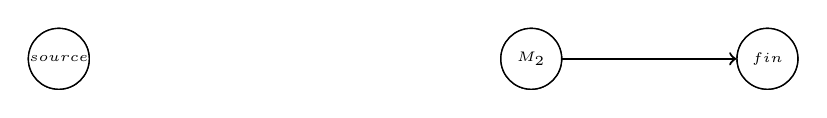
\begin{tikzpicture}[xscale=3, yscale=0.5, auto,swap]
 
    \foreach \pos/\name in {
	{(0,1)/source},
	{(2,1)/M_2},
	{(3,1)/fin}}
      \node[vertex] (\name) at \pos {$\name$};

    \foreach \source/ \dest in {M_2/fin} \path[edge] (\source) node[] {} -- node[] {} (\dest);
    
    \foreach \vertex in {source,M_2,fin}
        \path node[selected vertex] at (\vertex) {$\vertex$};
\end{tikzpicture}\\
Suppression de $M_1$\\

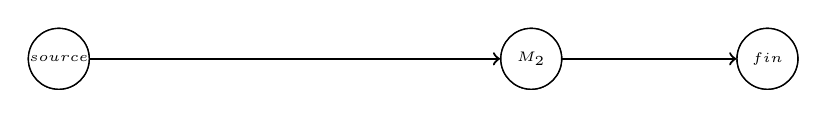
\begin{tikzpicture}[xscale=3, yscale=0.5, auto,swap]
    \foreach \pos/\name in {
	{(0,1)/source},
	{(2,1)/M_2},
	{(3,1)/fin}}
      \node[vertex] (\name) at \pos {$\name$};

    \foreach \source/ \dest in {source/M_2,M_2/fin} \path[edge] (\source) node[] {} -- node[] {} (\dest);
    
    \foreach \vertex in {source,M_2,fin}
        \path node[selected vertex] at (\vertex) {$\vertex$};
\end{tikzpicture}\\
Ajout de l'arc $(v_{source}, M_2)$\\

\caption{Suppression du sommet $M_1$ : ajout d'un arc entre les sommets $source$ et $M_2$}
\label{fig:suppressionSommet}
\end{figure}

Modélisé par un graphe complet, l'espace de recherche est immense. Un tel graphe permet de représenter toutes les solutions possibles au problème alors qu'une grande partie de ces solutions sont de très mauvaise qualité. Les informations apportées par les fenêtres de temps permettent pourtant d'explorer uniquement les solutions les plus performantes. 
Ainsi, il est possible de réduire la taille de l'espace de recherche en analysant le voisinage des n\oe{}uds dans le graphe. 
En effet, lorsqu'un n\oe{}ud est ajouté au graphe, il est possible de prendre en compte la notion de précédence entre les missions pour éviter la redondance des arcs dans le graphe.

Dans le cas décrit par la figure \ref{fig:suppressionRedondance}, où les arcs $(a,b)$, $(a,c)$ et $(b,c)$ se trouvent sur le graphe après l'ajout du sommet $b$, l'arc $(a,c)$ sera supprimé afin d'assurer que le véhicule réalisant la mission $a$ réalise ensuite la mission $b$ avant d'effectuer $c$. Sans cette suppression, le cas où $c$ serait réalisé avant $b$ serait envisagé. En effet, chaque mission étant supprimée du graphe lorsqu'elle est réalisée, la mission $b$ se trouverait réalisable après l'exécution de $a$ puis de $c$. Or, les fenêtres de temps permettent à un même véhicule de réaliser $a$, puis $b$, puis $c$ sans dépassement mais pas $a$ puis $c$ puis $b$.

\begin{figure}[h]
\centering
\tiny
\tikzstyle{vertex}=[circle,draw,fill=white,line width=0.5pt,minimum size=25pt,inner sep=0pt,font=\tiny]
\tikzstyle{selected vertex} = [vertex]
\tikzstyle{red vertex} = [vertex, fill=black!100, text=white]
\tikzstyle{blue vertex} = [vertex, fill=black!40]
\tikzstyle{edge} = [draw,thick,->]
\tikzstyle{weight} = [font=\tiny]
\tikzstyle{weightRed} = [font=\tiny, black!100]
\tikzstyle{weightBlue} = [font=\tiny, black!40]
\tikzstyle{red edge} = [draw,thick,->,red!100]
\tikzstyle{blue edge} = [draw,thick,->,blue!100]
\tikzstyle{ignored edge} = [draw,line width=5pt,-,black!20]
 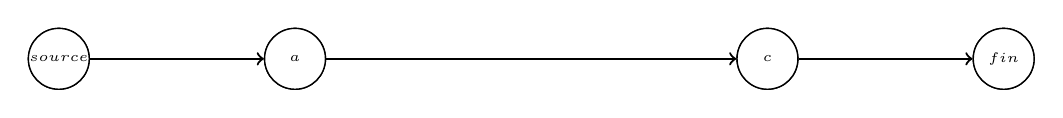
\begin{tikzpicture}[xscale=3, yscale=0.5, auto,swap]
 
    \foreach \pos/\name in {
	{(0,1)/source},
	{(1,1)/a}, {(3,1)/c},
	{(4,1)/fin}}
      \node[vertex] (\name) at \pos {$\name$};

    \foreach \source/ \dest in {source/a, a/c, c/fin} \path[edge] (\source) node[] {} -- node[] {} (\dest);
    
    \foreach \vertex in {source,a,c,fin}
        \path node[selected vertex] at (\vertex) {$\vertex$};
\end{tikzpicture}\\
Graphe initial\\

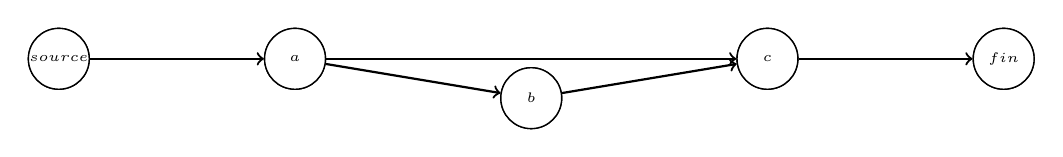
\begin{tikzpicture}[xscale=3, yscale=0.5, auto,swap]
 
    \foreach \pos/\name in {
	{(0,1)/source},
	{(1,1)/a}, {(2,0)/b}, {(3,1)/c},
	{(4,1)/fin}}
      \node[vertex] (\name) at \pos {$\name$};

    \foreach \source/ \dest in {source/a, a/b, a/c, b/c, c/fin} \path[edge] (\source) node[] {} -- node[] {} (\dest);
    
    \foreach \vertex in {source,a,b,c,fin}
        \path node[selected vertex] at (\vertex) {$\vertex$};
\end{tikzpicture}\\
Ajout de $b$\\

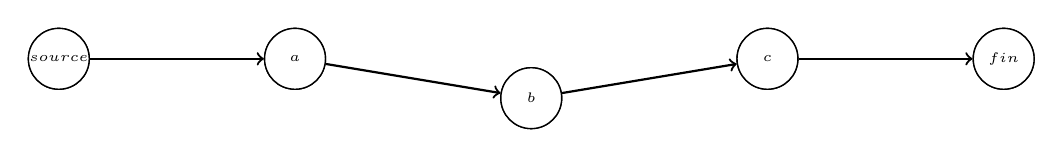
\begin{tikzpicture}[xscale=3, yscale=0.5, auto,swap]
 
    \foreach \pos/\name in {
	{(0,1)/source},
	{(1,1)/a}, {(2,0)/b}, {(3,1)/c},
	{(4,1)/fin}}
      \node[vertex] (\name) at \pos {$\name$};

    \foreach \source/ \dest in {source/a, a/b, b/c, c/fin} \path[edge] (\source) node[] {} -- node[] {} (\dest);
    
    \foreach \vertex in {source,a,b,c,fin}
        \path node[selected vertex] at (\vertex) {$\vertex$};
\end{tikzpicture}\\
Suppression de la redondance $(a,c)$\\
\caption{Suppression des arcs redondants}
\label{fig:suppressionRedondance}
\end{figure}

\paragraph{Gestion de la dynamique}

Dans la version dynamique du problème, les missions peuvent être insérées, annulées ou modifiées et le graphe doit être en mesure d'évoluer en fonction de ces modifications. De plus, la flotte de véhicules pouvant également être concerné par des événements dynamique (pannes, trafic, comportement humain...), les informations doivent être mises-à-jour sur le graphe afin de modéliser efficacement les colonies correspondantes.

Lorsqu'une nouvelle mission $i$ est insérée dans l'ordonnanceur, un noeud $v_i$ est ajouté au graphe. De nouveaux arcs reliant $v_i$ aux autres sommets du graphe sont créés en respectant la structure décrite dans le paragraphe précédent. Si l'insertion de $v_i$ dans le graphe conduit à la création de deux arcs $(v_{source},v_i)$ et $(v_i,v_j)$ et si l'arc $(v_{source}, v_j)$ existe déjà, alors ce dernier doit être supprimé. Le procédé est le même concernant le noeud de fin. Cette procédure est nécessaire pour obliger les véhicules à effectuer chaque mission. Dans le cas contraire, la meilleure solution trouvée par l'algorithme consisterait à n'effectuer aucune mission car ainsi la fonction d'évaluation serait nulle et donc minimale.

Lorsqu'une mission est annulée ou terminée, le sommet correspondant doit être retiré du graphe. Ses arcs incidents sont alors également supprimés, mais il est possible que de nouveaux arcs doivent être ajoutés afin de connecter les prédécesseurs du n\oe{}ud supprimé à ses successeurs, en suivant les règles décrites précédemment.

Quand une mission est mise-à-jour, le sommet correspondant ainsi que ses arcs incidents sont supprimés du graphe. Puis le noeud est inséré de nouveau et les nouveaux arcs créés prennent ainsi en compte les nouvelles caractéristiques de la mission.

Quand un véhicule commence à réaliser une mission, il doit la mener à son terme à moins de tomber en panne. Dans ce dernier cas, la mission doit être mise-à-jour car le point de collecte du conteneur peut avoir changé si le véhicule avait commencé à déplacer le conteneur avant de tomber en panne. 
Si le véhicule devient indisponible, les fourmis de la colonie correspondante sont réinitialisées au sommet source et doivent y rester tant que le véhicule ne redevient pas disponible. Dans le même temps, le processus d'évaporation aura fait disparaître progressivement la phéromone de cette colonie permettant ainsi aux autres colonies de coloniser les missions concernées.

Si le véhicule ne tombe pas en panne, il doit achever sa mission. Pour représenter cette contrainte les fourmis de la colonie du véhicule débutent leur parcourt depuis le n\oe{}ud de la mission courante. La phéromone des autres fourmis sur ce noeud est évaporée afin de le rendre inaccessible aux autres colonies.

\paragraph{Gestion de la phéromone}

La phéromone permet d'indiquer aux individus quels ont été les choix réalisés par d'autres fourmis et également quel fut la qualité du chemin construit en suivant ces choix. L'utilisation de phéromone colorée permet de répartir les individus sur le graphe des missions et ainsi de distribuer les tâches aux différentes ressources. 
Un système de dépôt de phéromone sur les arcs du graphe permet de retracer le chemin complet d'une fourmi du n\oe{}ud source au n\oe{}ud fin. Toutefois, un tel système ne permet pas de faire fonctionner le mécanisme de compétition entre les colonies.
En effet, un sommet peu être atteint par une fourmi à partir de chacun de ses arcs entrants. Il existe ainsi plusieurs chemins menant à un sommet. Des fourmis de colonies différentes peuvent ainsi accéder à un sommet par des chemin différents sans être repoussées par la phéromone étrangère.

Le système utilisé ici consiste à déposer de la phéromone sur les sommets du graphe au lieu des arcs. Ainsi, lorsqu'un sommet est atteint par une fourmi, les différentes phéromones sont prises en compte, peu importe la provenance de la fourmi. Ce procédé à en revanche l'inconvénient d'empêcher de retracer le chemin complet d'une fourmi du n\oe{}ud source au n\oe{}ud fin, c'est pourquoi les missions ne peuvent pas être affectées en prenant en compte les chemins dans le graphe.
Chaque affectation sera donc uniquement déterminée par la couleur dominante de la phéromone sur le sommet correspondant à la mission à affecter.

Par exemple, le graphe de la figure \ref{fig:grapheDeMission} reprend les données de l'exemple de la figure \ref{fig:exempleJSSP} et montre la coloration du graphe par les deux colonies de fourmis. Ici, la phéromone de la colonie du véhicule $V_1$ est majoritaire sur le sommet $M_2$ alors que la phéromone de la colonie du véhicule $V_2$ est majoritaire sur les n\oe{}uds $M_1$ et $M_3$. La figure indique également l'évolution du graphe dans le temps. À l'initialisation la structure du graphe indique bien que $M_1$ et $M_2$ ne peuvent pas être enchaînées par un même véhicule. La colonisation du graphe par les fourmis permet de distribuer les missions aux chariots cavaliers qui ensuite les exécutent. Ainsi, d'abord $M_2$ est réalisée par $V_2$, puis parallèlement $M_1$ est exécutée par $V_1$. Enfin, $V_2$ effectue la mission $M_3$.

\begin{figure}[h]
 \centering
 \tiny
 \tiny
\tikzstyle{vertex}=[circle,draw,fill=white,line width=0.5pt,minimum size=22pt,inner sep=0pt,font=\tiny]
\tikzstyle{selected vertex} = [vertex]
\tikzstyle{red vertex} = [vertex, fill=black!100, text=white]
\tikzstyle{blue vertex} = [vertex, fill=black!40]
\tikzstyle{edge} = [draw,thick,->]
\tikzstyle{weight} = [font=\tiny]
\tikzstyle{weightRed} = [font=\tiny, black!100]
\tikzstyle{weightBlue} = [font=\tiny, black!40]
\tikzstyle{red edge} = [draw,thick,->,red!100]
\tikzstyle{blue edge} = [draw,thick,->,blue!100]
\tikzstyle{ignored edge} = [draw,line width=5pt,-,black!20]

\begin{tabular}{rl}

\multicolumn{2}{c}{
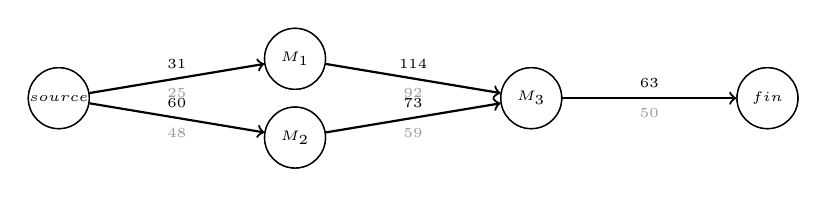
\begin{tikzpicture}[xscale=3, yscale=0.5, auto,swap]
    \foreach \pos/\name in {
	{(0,1)/source},
	{(1,2)/M_1}, {(1,0)/M_2},
	{(2,1)/M_3},
	{(3,1)/fin}}
      \node[vertex] (\name) at \pos {$\name$};

    \foreach \source/ \dest /\weightRed/\weightBlue in {source/M_1/31/25, source/M_2/60/48, M_1/M_3/114/92, M_2/M_3/73/59, M_3/fin/63/50} \path[edge] (\source) -- node[weightRed,above] {$\weightRed$} node[weightBlue,below]{$\weightBlue$} (\dest);
    
    \foreach \vertex in {source,fin,M_1,M_2,M_3}
        \path node[selected vertex] at (\vertex) {$\vertex$};
\end{tikzpicture}} \\
\vspace{1pt}
t=$00:00:00$ & Graphe initial.\\
\multicolumn{2}{c}{
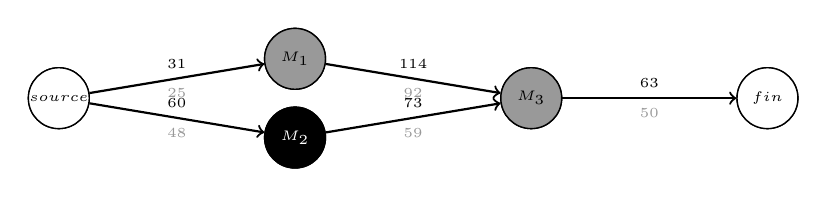
\begin{tikzpicture}[xscale=3, yscale=0.5, auto,swap]
    \foreach \pos/\name in {
	{(0,1)/source},
	{(1,2)/M_1}, {(1,0)/M_2},
	{(2,1)/M_3},
	{(3,1)/fin}}
      \node[vertex] (\name) at \pos {$\name$};

    \foreach \source/ \dest /\weightRed/\weightBlue in {source/M_1/31/25, source/M_2/60/48, M_1/M_3/114/92, M_2/M_3/73/59, M_3/fin/63/50} \path[edge] (\source) -- node[weightRed,above] {$\weightRed$} node[weightBlue,below]{$\weightBlue$} (\dest);
    
    \foreach \vertex in {source,fin}
        \path node[selected vertex] at (\vertex) {$\vertex$};
    \foreach \vertex in {M_2}
        \path node[red vertex] at (\vertex) {$\vertex$};
    \foreach \vertex in {M_1,M_3}
        \path node[blue vertex] at (\vertex) {$\vertex$};
\end{tikzpicture}} \\
\vspace{1pt}
t=$00:00:00$ & Graphe pondéré et coloré après colonisation par les fourmis. \\


\multicolumn{2}{c}{
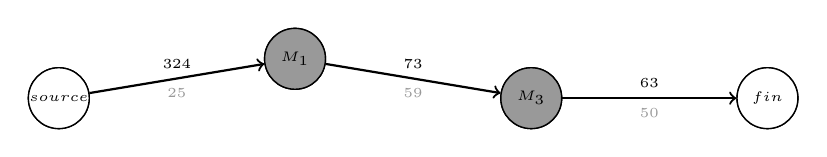
\begin{tikzpicture}[xscale=3, yscale=0.5, auto,swap]
    \foreach \pos/\name in {
	{(0,1)/source},
	{(1,2)/M_1},
	{(2,1)/M_3},
	{(3,1)/fin}}
      \node[vertex] (\name) at \pos {$\name$};

    \foreach \source/ \dest /\weightRed/\weightBlue in {source/M_1/324/25, M_1/M_3/73/59, M_3/fin/63/50} \path[edge] (\source) -- node[weightRed,above] {$\weightRed$} node[weightBlue,below]{$\weightBlue$} (\dest);
    
    \foreach \vertex in {source,fin}
        \path node[selected vertex] at (\vertex) {$\vertex$};
    \foreach \vertex in {M_1,M_3}
        \path node[blue vertex] at (\vertex) {$\vertex$};
\end{tikzpicture}}\\
\vspace{1pt}
t=$00:00:32$ & début de l'exécution de $M_2$ par $V_1$.\\ 
\multicolumn{2}{c}{
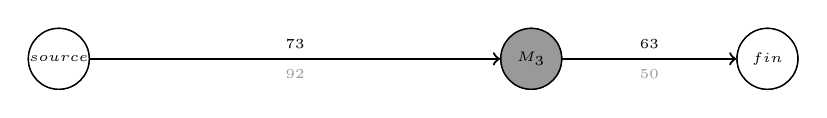
\begin{tikzpicture}[xscale=3, yscale=0.5, auto,swap]
    \foreach \pos/\name in {
	{(0,1)/source},
	{(2,1)/M_3},
	{(3,1)/fin}}
      \node[vertex] (\name) at \pos {$\name$};

    \foreach \source/ \dest /\weightRed/\weightBlue in {source/M_3/73/92, M_3/fin/63/50} \path[edge] (\source) -- node[weightRed,above] {$\weightRed$} node[weightBlue,below]{$\weightBlue$} (\dest);
    
    \foreach \vertex in {source,fin}
        \path node[selected vertex] at (\vertex) {$\vertex$};
    \foreach \vertex in {M_3}
        \path node[blue vertex] at (\vertex) {$\vertex$};
\end{tikzpicture}}\\
\vspace{1pt}
t=$00:00:34$ & début de l'exécution de $M_1$ par $V_2$.\\
\multicolumn{2}{c}{
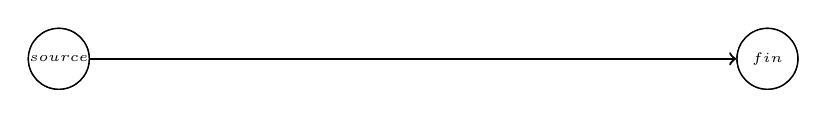
\begin{tikzpicture}[xscale=3, yscale=0.5, auto,swap]
    \foreach \pos/\name in {
	{(0,1)/source},
	{(3,1)/fin}}
      \node[vertex] (\name) at \pos {$\name$};

    \foreach \source/ \dest in {source/fin} \path[edge] (\source) -- (\dest);
    
    \foreach \vertex in {source,fin}
        \path node[selected vertex] at (\vertex) {$\vertex$};    
\end{tikzpicture}}\\
\vspace{1pt}
t=$00:06:47$ & Début de l'exécution de $M_3$ par $V_2$. \\
\multicolumn{2}{c}{
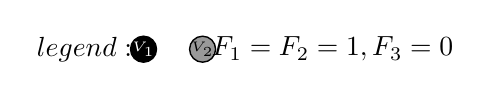
\begin{tikzpicture}[xscale=3, yscale=0.5, auto,swap]
\node[minimum size=5pt] (legend) at (1.25,-1) {$legend:$};    
\node[red vertex, minimum size=5pt] (v1legend) at (1.5,-1) {$V_1$};    
\node[blue vertex, minimum size=5pt] (v2legend) at (1.75,-1) {$V_2$};
\node[minimum size=5pt] (fValues) at (2.3,-1) {$F_1 = F_2 = 1, F_3 = 0$};
\end{tikzpicture}}\\
\end{tabular}
 \caption{Graphe dynamique de l'exemple de la figure \ref{fig:exempleJSSP} (voir p.\pageref{fig:exempleJSSP})}
 \label{fig:grapheDeMission}
\end{figure}

Hormis l'emplacement de dépôt de la phéromone, le fonctionnement reste identique à celui de l'algorithme hors-ligne. Ainsi il y a deux mécanismes : l'un de renforcement (\textit{positive feedback}) et l'autre d'évaporation (\textit{negative feedback}). L'équation \ref{eq:acoContinu:renforcement} décrit la quantité de phéromone déposée par la fourmi $k$ sur le sommet $j$ en venant de $i$ au temps $t$ et l'équation \ref{eq:acoContinu:pheromone} indique la quantité de phéromone de la couleur de la fourmi $k$ qui sera présente sur le sommet $i$ au temps $t$. 

\begin{equation}\label{eq:acoContinu:renforcement}
 \Delta^k_{ij}(t) = \frac{1}{c^k_{ij}(t)}
\end{equation}

\begin{equation}\label{eq:acoContinu:pheromone}
 \tau^k_{j}(t) = \max \left(\lambda , \rho \cdot \tau^k_{j}(t-1) \right) + \sum\limits_{i \in P_j}\left(\Delta^k_{ij}(t)\right)
\end{equation}

La quantité de phéromone présente sur un sommet $i$ au temps $t$ de couleur différente de celle de la colonie $k$ est décrite par l'équation suivante : 

\begin{equation}
  \hat \tau^k_{i}(t) = \left( \sum \limits_{l=1, l \neq k}^{m} (\tau^l_{i}(t)) \right)
\end{equation}

\paragraph{Règle de transition pseudo-aléatoire proportionnelle}

La règle de transition reste identique à celle utilisée par l'algorithme hors-ligne, mis à part l'emplacement de la phéromone qui se trouve dorénavant sur les sommets. Une fourmi choisit donc aléatoirement une mission à réaliser parmi les missions non-affectées selon les probabilités calculées par l'équation \ref{eq:acoContinu:transition}. 

\begin{equation} \label{eq:acoContinu:transition}
 p^k_{ij}(t) = \frac{\bigg[\tau^k_{j}(t)\bigg]^\alpha \cdot \bigg[1 + \frac{1}{c^k_{ij}(t)}\bigg]^\beta \cdot \bigg[1 + \frac{\tau^k_{j}(t)}{\sum \limits_{l=1}^{m} \tau^l_{j}(t)}\bigg]^\gamma}
 {\sum \limits_{s \in S_i} \left(\bigg[\tau^k_{s}(t)\bigg]^\alpha \cdot \bigg[1 + \frac{1}{c^k_{is}(t)}\bigg]^\beta \cdot \bigg[1 + \frac{\tau^k_{s}(t)}{\sum \limits_{l=1}^{m} \tau^l_{s}(t)}\bigg]^\gamma\right)}
\end{equation}

Afin d'empêcher la colonisation continue du graphe par les colonies il est nécessaire de déterminer un seuil d'acceptation de la transition. En effet, si il existe dans le problème plus de véhicules que de missions à affecter, alors il est impossible d'attribuer une mission à chaque véhicule. Ce seuil est fixé par la constante $\Delta$. Si la probabilité de la destination choisie est inférieure à $\Delta$, alors la fourmi est replacée sur le n\oe{}ud source.

\paragraph{Solution \textit{anytime}}

À n'importe quel moment les plans de charge calculés par l'algorithme peuvent-être obtenus. Ainsi la solution est constituée de $m$ chemins dans le graphe de différentes couleurs. Le graphe des missions étant orienté et acyclique, chaque chemin peut-être reconstruit en partant du n\oe{}ud source et en choisissant parmi les sommets accessibles colorés par la même couleur que le chemin construit, celui qui possède la plus grande quantité de phéromone. La construction est complète lorsque le n\oe{}ud fin est atteint ou lorsqu'aucun sommet de la couleur du chemin n'est accessible.

\paragraph{Renforcement du chemin courant}

Lorsqu'un véhicule commence à réaliser une mission d'un chemin, un processus de renforcement de la piste de phéromone de la couleur de la colonie du véhicule intervient sur la totalité du chemin. La trace de phéromone de cette couleur est augmentée afin d'empêcher que la couleur des sommets change trop rapidement pendant que la solution précédemment calculée est réalisée. Les sommets concernés deviennent moins attractifs pour les autres colonies. La constante $\Lambda$ définit ainsi la quantité de renforcement et le processus suit l'algorithme \ref{algo:acoContinu:renforcement}.

\begin{algorithm}[H]

\Deb{
\PourCh{ sommet i du chemin} {
  $\tau^k_{i}(t) = \tau^k_{i}(t-1) + \Lambda$
}
}
\caption{Renforcement du chemin d'une solution en cours de réalisation}
\label{algo:acoContinu:renforcement}
\end{algorithm}

\paragraph{Algorithme général}

L'algorithme principal (voir Algorithme \ref{algo:acoContinu}) prend en paramètre la liste des véhicules ainsi et que le graphe des missions à ordonnancer et à affecter. À chaque itération de l'algorithme, chaque fourmi de chaque colonie choisie une destination parmi les sommets voisins de sa position courante sur le graphe. Elle retourne au n\oe{}ud source si aucun voisin n'est accessible, ou dans le cas contraire se rend sur le sommet choisit et y dépose de la phéromone. Après que chaque fourmi de chaque colonie se soit déplacée, le processus d'évaporation est effectué et les solutions sont mises-à-jour.

\begin{algorithm}[H]
\Donnees{\\
\begin{tabular}{l}
 M : liste des véhicules,\\
 V : sommets du graphe,\\
 A : arcs du graphe
\end{tabular}} 
\Deb{
   \PourCh{fourmi $f$ de chaque colonie $k$}{
     destination $\leftarrow$ choisir\_destination(f)\;
     position\_courante $\leftarrow$ position(f)\;
     \eSi{destination $= \emptyset$}{
       retourner\_au\_noeud\_source(f)\;
     }{
       deplacement(f,destination)\;
       deposer\_pheromone(f,position\_courante,destination)\;
     }
   }
    \PourCh{sommet v $\in$ V}{
       evaporation(v)\;
    }
    \PourCh{colonie k}
    {
      mise\_a\_jour\_chemin(k)\;
    }
}
\caption{méthode de résolution dynamique en-ligne}
\label{algo:acoContinu}
\end{algorithm}

\paragraph{Paramètres}

L'algorithme de résolution en-ligne reprend tous les paramètres de la méthode hors-ligne à l'exception de $\Theta$ qui était utilisé dans l'autre méthode pour définir le nombre d'itérations à réaliser. Ici, il n'est plus question de limiter le temps de calcul mais bien de calculer en continu les solutions. Trois autres paramètres sont nécessaires au fonctionnement de cette méthode. D'abord $\eta$ qui définit le nombre d'individus à utiliser par colonie. Ensuite $\Delta$ qui modélise la pression de l'environnement en forçant la fourmi à mourir si la part de sa phéromone présente sur le noeud choisit est trop faible. Enfin, $\Lambda$ sert à définir la quantité de phéromone déposée sur un chemin lorsqu'une mission de celui-ci est commencée par un véhicule.

On peut distinguer, dans la liste ci-dessous, deux classes de paramètres : d'une part ceux qui concernent le choix de la destination pour la fourmi ($\alpha$, $\beta$, $\gamma$, $\Delta$, $F_1$, $F_2$ et $F_3$), et d'autre part ceux qui régissent la gestion de la phéromone ($\lambda$, $\Lambda$ et $\rho$).\\

\begin{tabular}{ccp{0.9\textwidth}}
 $\alpha$ &:& importance relative de la trace de phéromone lors du choix de la destination;\\
 $\beta$ &:& importance relative de l'heuristique de pondération lors du choix de la destination;\\
 $\gamma$ &:& importance relative du processus de répulsion lors du choix de la destination;\\
 $\eta$ &:& nombre de fourmis par colonie;\\
 $\Delta$ &:& pression de l'environnement;\\
 $\lambda$ &:& quantité minimale de phéromone présente sur chaque arc;\\
 $\Lambda$ &:& quantité de phéromone de renforcement de chemin;\\
 $\rho$ &:& taux de conservation de la phéromone après chaque itération de l'algorithme;\\
 $F_1$ &:& importance relative de la durée des trajets dans l'évaluation de l'enchaînement de deux missions;\\
 $F_2$ &:& importance relative du retard pondéré dans l'évaluation de l'enchaînement de deux missions;\\
 $F_3$ &:& importance relative de l'avance dans l'évaluation de l'enchaînement de deux missions;\\
 $F_1'$ &:& importance relative de la durée des trajets dans l'évaluation globale d'une solution;\\
 $F_2'$ &:& importance relative du retard pondéré dans l'évaluation globale d'une solution;\\
 $F_3'$ &:& importance relative de l'avance dans l'évaluation globale d'une solution.
\end{tabular}